\chapter{Evaluation of MIBot}
\label{ch:mibot-eval}

This chapter presents a comprehensive evaluation of MIBot's effectiveness through a \margindex{Feasibility Study}feasibility study with 106 smokers. Building on the system design and implementation described in previous chapters, we assess MIBot's performance across four critical dimensions established in the smoking cessation and motivational interviewing literature: behavioural change readiness, \margindex{Perceived Therapeutic Empathy}[Perceived Empathy]perceived therapeutic empathy, \margindex{MI Adherence}[MI Adherence]adherence to MI principles, and elicitation of client change talk.

The chapter is organized to progress from primary outcomes through measurements of therapeutic process, and finally, to behavioural changes and user experiences. First, we report the primary outcome of changes in readiness to quit smoking (Section~\ref{sec:primary-outcome}). We then analyze how chatbot performed on perceived empathy, measured through the CARE scale and compare it to human healthcare professionals (Section~\ref{sec:perceived-empathy}). Next, we examine MIBot's adherence to MI principles through AutoMISC analysis, and examine if MIBot could maintain fidelity to therapeutic standards while successfully eliciting change talk from clients (Section~\ref{sec:mi-adherence}).

Following these core metrics, we investigate behavioural outcomes including quit attempts and self-reported changes (Section~\ref{sec:behavioural-outcomes}), explore conversation dynamics both quantitatively and qualitatively (Section~\ref{sec:conversation-dynamics}), and examine illustrative case studies and sample outliers (Section~\ref{sec:case-studies}). Finally, we analyze participant feedback (Section~\ref{sec:feedback}) and discuss broader implications of our findings (Section~\ref{sec:synthesis}).

\section{Primary Outcome: Readiness to Quit}
\label{sec:primary-outcome}

\subsection{Overall Changes in Readiness Rulers}

Table~\ref{table:mibot_ruler_summary} summarizes the mean (and standard deviation) of each readiness ruler before the conversation, immediately afterwards, and one week later.   The table includes the change between the pre-conversation metric and one week later ($\Delta$). The Wilcoxon signed-rank test was applied to assess the significance of the change. Participants' confidence increased markedly from a baseline mean of 2.8 to 4.5 one week later ($\Delta=1.66$, $p<10^{-9}$). This represents a $\sim$59\% relative improvement and constitutes our \margindex{Primary Outcome}[Primary Outcome]primary outcome measure, aligning with MI theory that confidence (self-efficacy) is a key predictor of behaviour change \citep{Gwaltney2009-wj,Abar2013}. Importance also increased, albeit more modestly ($\Delta=0.5$, $p<0.005$), while readiness exhibited a small, non-significant change ($\Delta=0.23$, $p=0.22$).

\begin{table}[ht!]
  \centering
  \small
  \setlength{\tabcolsep}{4pt}
  \renewcommand{\arraystretch}{1.1}
  \begin{tabular}{@{}lcccc@{}}
    \toprule
    \textbf{Ruler} & \textbf{Before} & \textbf{After} & \textbf{One Week} & \textbf{$\Delta$} \\
    & \textbf{mean (SD)} & \textbf{mean (SD)} & \textbf{mean (SD)} & \textbf{mean (SD)} \\
    \midrule
    Importance & 5.7 (2.6) & 6.3 (2.9) & 6.1 (2.7) & 0.5 (1.7)** \\
    Confidence & 2.8 (2.0) & 4.6 (2.6) & 4.5 (2.7) & 1.7 (2.4)*** \\
    Readiness  & 5.2 (2.8) & 5.9 (2.8) & 5.5 (3.0) & 0.3 (2.4) \\
    \bottomrule
  \end{tabular}
  \caption{Means (SD) of readiness rulers (0--10 scale) before the conversation, immediately after, one week later, and the week-later change ($\Delta$). SD = standard deviation. Wilcoxon signed-rank test: *** $p < 0.001$, ** $p < 0.01$, * $p < 0.05$, n.s. = not significant ($p \geq 0.05$).}
  \label{table:mibot_ruler_summary}
\end{table}

Figure~\ref{fig:confidence_change_distribution} illustrates the distribution of one-week changes in confidence. Of the 106 participants, 64 (60.4\%) showed improvement, 21 (19.8\%) remained unchanged, and 21 (19.8\%) experienced a decrease. The median change was +1.0 point, with the interquartile range spanning 0 to +3 points. Notably, 15 participants (14.2\%) achieved gains of 5 or more points, representing substantial movement toward quitting confidence.

\begin{figure}[ht]
  \centering
  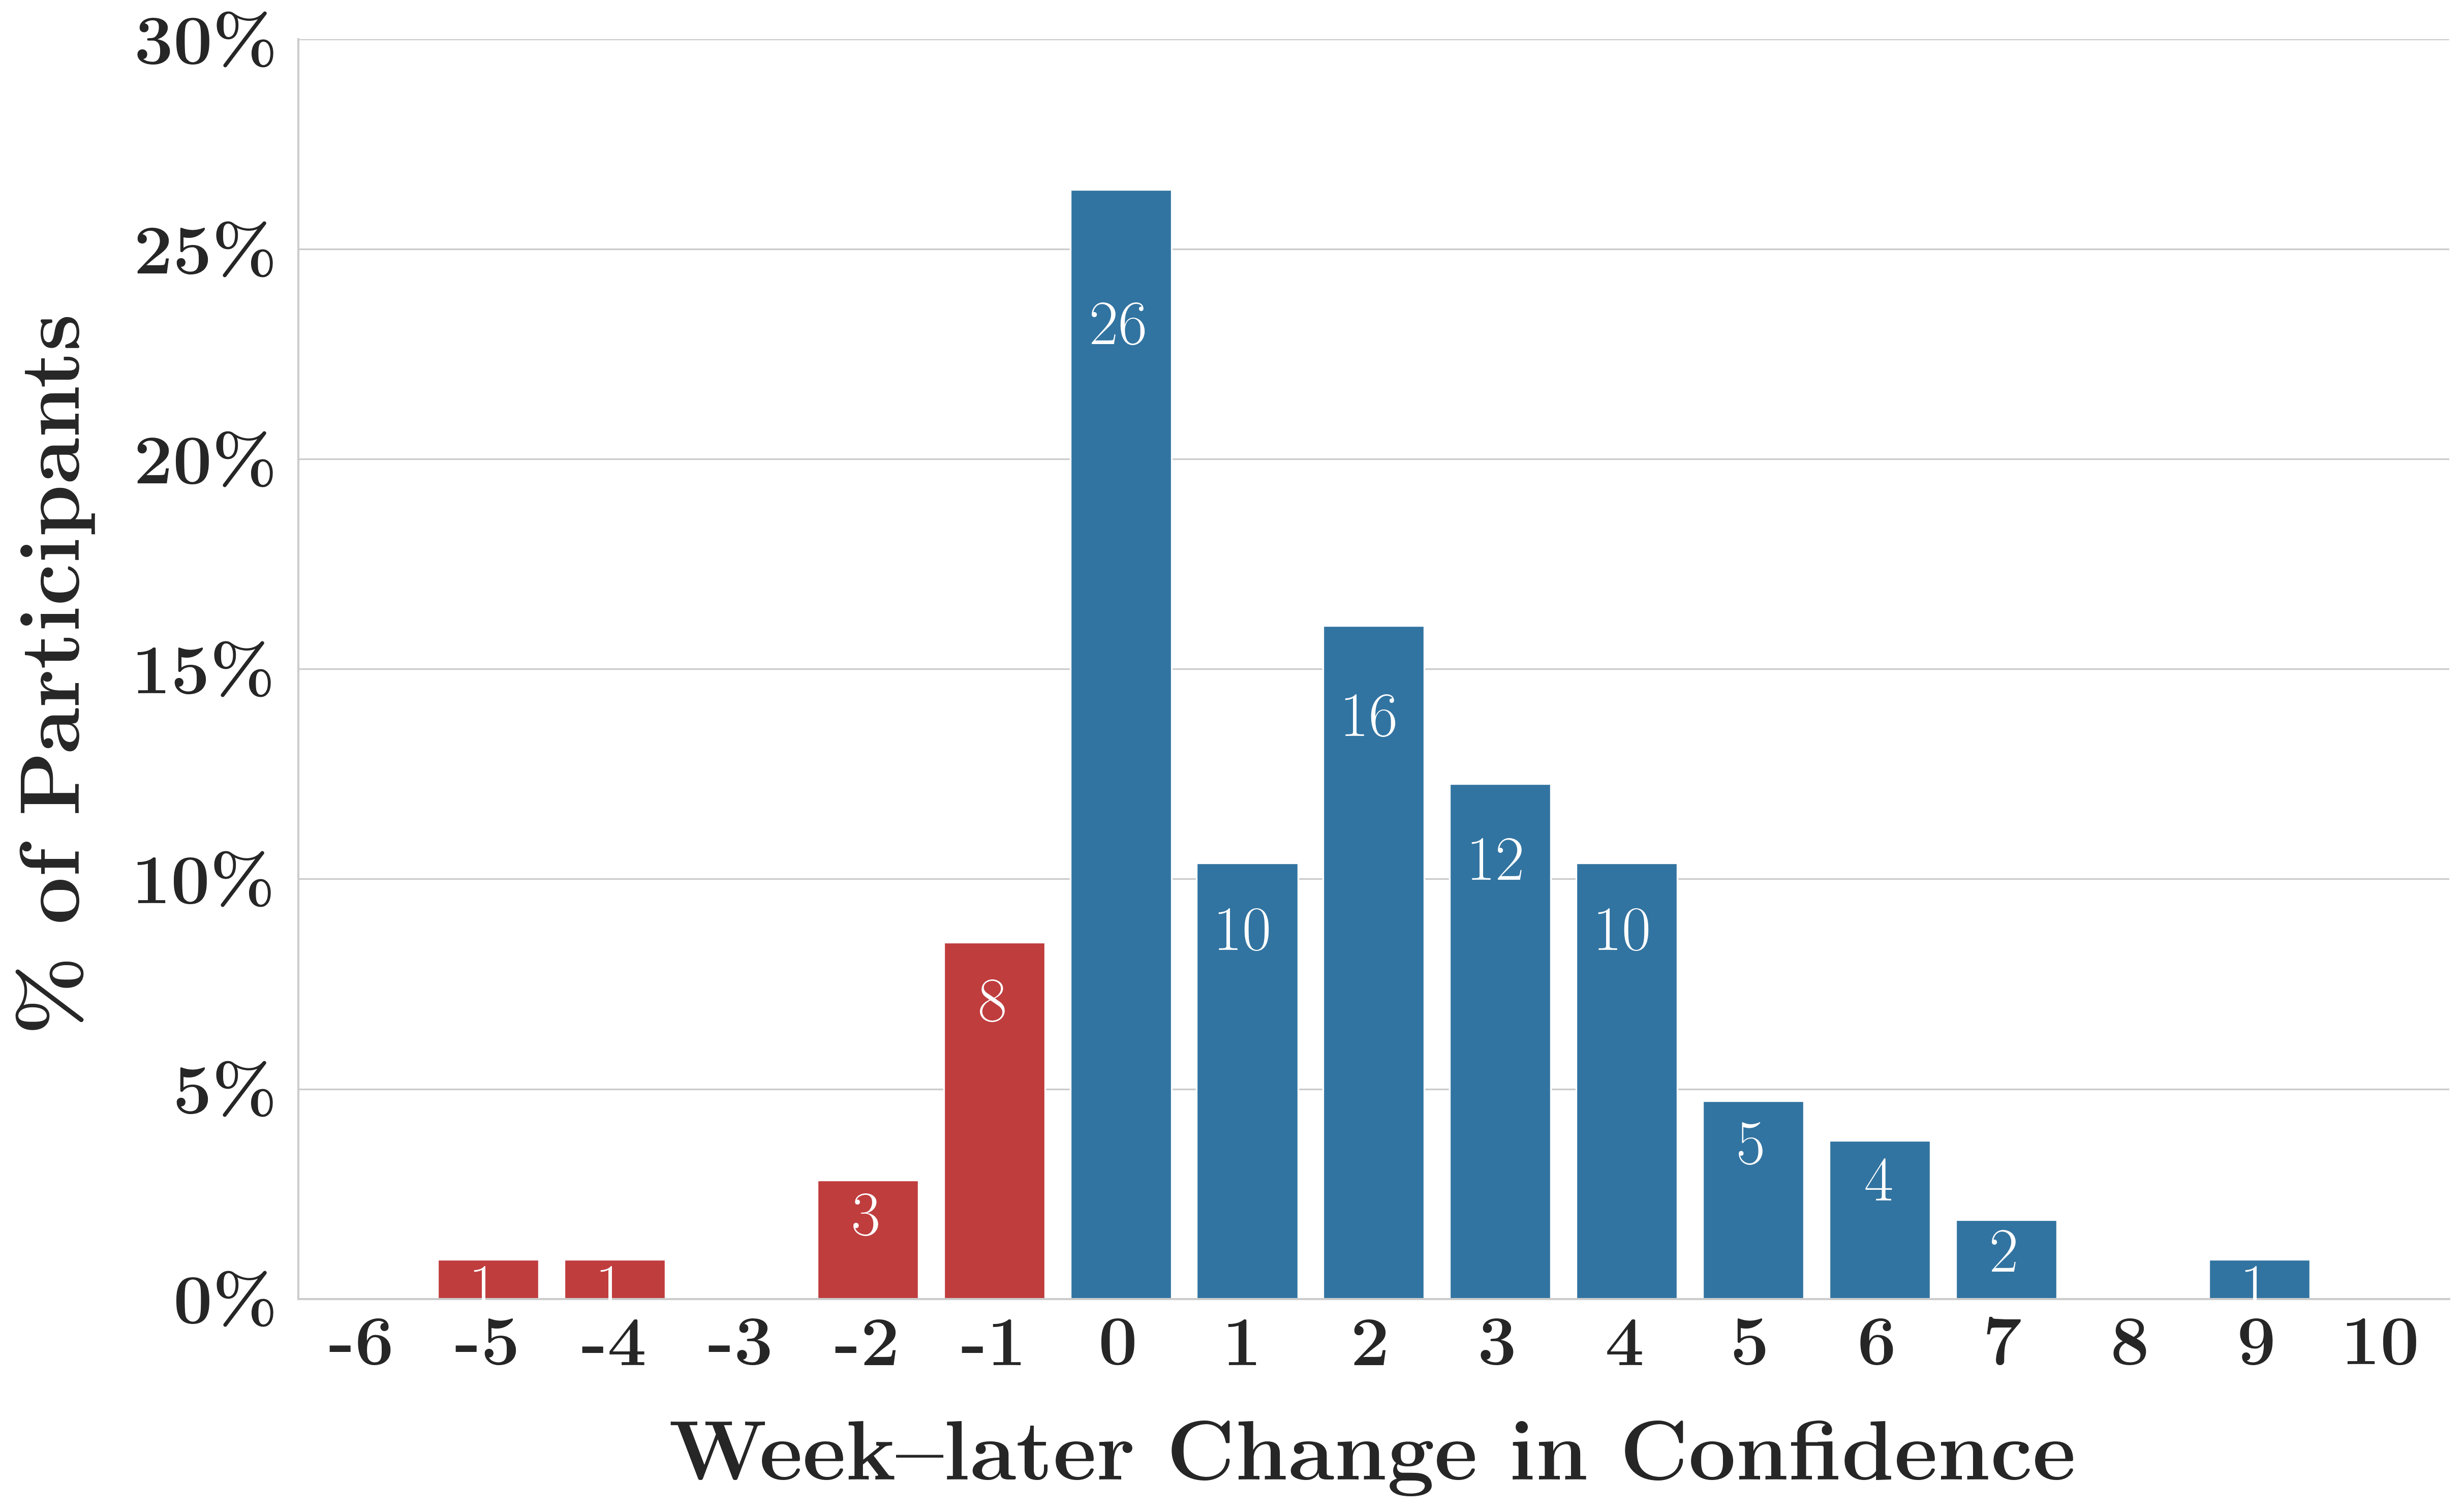
\includegraphics[width=0.8\linewidth]{fig/2024-11-14-MIV6.3A-2024-11-22-MIV6.3A_ruler_deltas_delta_with_week_later_keep_high_conf_False_change.png}
  \caption{Distribution of one-week changes in confidence scores. The majority of participants (60.4\%) showed improvement, with a long right tail indicating some participants experienced dramatic gains.}
  \label{fig:confidence_change_distribution}
\end{figure}



\subsection{Stratified Analysis by Baseline Characteristics}

To understand which participants benefited most from MIBot, we stratified outcomes by baseline characteristics. Table~\ref{tab:baseline_confidence} shows that those starting with the lowest self-confidence ($n=31$, confidence $\leq 1$) experienced the largest improvement (+2.2 points), whereas participants with moderate or higher confidence gained about one and a half points. The three participants who began with very high confidence showed a decline, likely reflecting \margindex{Regression To The Mean}[Regression to Mean]regression to the mean. Baseline confidence correlated negatively with the change (Spearman $r=-0.21$, $p<0.05$), indicating that MIBot is most beneficial for participants who are least confident in their ability to quit.

\begin{table}[ht!]
  \centering
  \small
  \renewcommand{\arraystretch}{1.1}
  \begin{tabular*}{\linewidth}{@{\extracolsep{\fill}}lccccc@{}}
    \toprule
    \textbf{Baseline} & \textbf{Sample} & \textbf{Baseline} & \textbf{Post-} & \textbf{1-week} & \textbf{Change from} \\
    \textbf{confidence range} & \textbf{size} & \textbf{confidence} & \textbf{conversation} & \textbf{follow-up} & \textbf{baseline} \\
    & & \textbf{mean (SD)} & \textbf{mean} & \textbf{mean (SD)} & \textbf{mean (SD)} \\
    \midrule
    0--1   & 31 & 0.5 (0.5) & 2.7 & 2.7 (2.5) & +2.2 (2.4)*** \\
    2--3   & 32 & 2.5 (0.5) & 2.0 & 4.2 (2.6) & +1.7 (2.5)** \\
    4--5   & 40 & 4.3 (0.5) & 1.4 & 5.8 (2.0) & +1.5 (2.1)*** \\
    $\geq$6 & 3 & 9.3 (0.6) & 0.6 & 7.7 (3.2) & $-1.7$ (2.9) \\
    \bottomrule
  \end{tabular*}
  \caption{Longitudinal changes in self-reported confidence scores (0--10 scale) stratified by baseline confidence level. Values assessed at baseline (pre-conversation), immediately post-conversation, and at 1-week follow-up. Participants were grouped by their initial confidence scores. Change scores represent the difference between baseline and 1-week follow-up assessments. SD = standard deviation. Wilcoxon signed-rank test: *** $p < 0.001$, ** $p < 0.01$, * $p < 0.05$, n.s. = not significant ($p \geq 0.05$).}
  \label{tab:baseline_confidence}
\end{table}




Confidence changes varied across different smoking characteristics and quit history profiles. Participants were grouped by HSI (low 0--1, moderate 2--3, high 4--5, very high $\geq$ 6), daily cigarette consumption ($<$5, 5--9, 10--19, $\geq$20), whether they had made a quit attempt in the week before the study, and the number of prior attempts (0, 1--2, $\geq$3). The mean change in confidence for each subgroup is summarized in Table~\ref{tab:hsi_prequit}.

\begin{table}[ht!]
  \centering
  \small
  \renewcommand{\arraystretch}{1.1}
  \begin{tabular*}{\linewidth}{@{\extracolsep{\fill}}lccccc@{}}
    \toprule
    \textbf{Participant} & \textbf{Sample} & \textbf{Baseline} & \textbf{Post-} & \textbf{1-week} & \textbf{Change from} \\
    \textbf{characteristics} & \textbf{size} & \textbf{confidence} & \textbf{conversation} & \textbf{follow-up} & \textbf{baseline} \\
    & & \textbf{mean (SD)} & \textbf{mean (SD)} & \textbf{mean (SD)} & \textbf{mean (SD)} \\
    \midrule
    \multicolumn{6}{l}{\textit{Heaviness of Smoking Index}} \\
    \quad Low (0--1) & 28 & 3.5 (1.9) & 5.5 (2.3) & 4.9 (2.5) & +1.5 (2.7)** \\
    \quad Moderate (2--3) & 55 & 2.7 (2.0) & 4.1 (2.6) & 4.7 (2.9) & +2.0 (2.3)*** \\
    \quad High (4--5) & 21 & 2.5 (1.8) & 4.5 (2.3) & 3.3 (2.4) & +0.8 (2.1) \\
    \quad Very high ($\geq$6) & 2 & 1.5 (2.1) & 4.0 (5.7) & 5.0 (2.8) & +3.5 (0.7) \\
    \midrule
    \multicolumn{6}{l}{\textit{Daily cigarette consumption}} \\
    \quad $<$5 & 5 & 3.2 (1.3) & 5.2 (2.0) & 4.2 (2.6) & +1.0 (1.6) \\
    \quad 5--9 & 32 & 3.5 (2.5) & 5.2 (2.7) & 5.2 (3.0) & +1.7 (2.9)** \\
    \quad 10--19 & 38 & 2.8 (1.5) & 4.2 (2.5) & 4.5 (2.8) & +1.7 (2.1)*** \\
    \quad $\geq$20 & 31 & 2.1 (1.6) & 4.2 (2.5) & 3.7 (2.3) & +1.7 (2.3)*** \\
    \midrule
    \multicolumn{6}{l}{\textit{Pre-conversation quit attempt}} \\
    \quad Yes & 34 & 3.1 (1.6) & 5.1 (2.7) & 5.7 (2.6) & +2.6 (2.2)*** \\
    \quad No & 72 & 2.7 (2.1) & 4.3 (2.5) & 3.9 (2.6) & +1.2 (2.3)*** \\
    \midrule
    \multicolumn{6}{l}{\textit{Number of prior attempts}} \\
    \quad 0 & 72 & 2.7 (2.1) & 4.3 (2.5) & 3.9 (2.6) & +1.2 (2.3)*** \\
    \quad 1--2 & 16 & 3.3 (1.6) & 6.1 (2.5) & 6.9 (2.4) & +3.6 (2.0)*** \\
    \quad $\geq$3 & 18 & 2.8 (1.7) & 4.3 (2.6) & 4.7 (2.4) & +1.8 (2.0)** \\
    \bottomrule
  \end{tabular*}
  \caption{Longitudinal changes in quit confidence scores stratified by baseline smoking characteristics and quit history. Values represent self-reported confidence to quit smoking (0--10 scale) assessed at baseline (pre-conversation), immediately post-conversation, and at 1-week follow-up. Change scores represent the difference between baseline and 1-week follow-up assessments. SD = standard deviation. Wilcoxon signed-rank test: *** $p < 0.001$, ** $p < 0.01$, * $p < 0.05$, n.s. = not significant ($p \geq 0.05$).}
  \label{tab:hsi_prequit}
\end{table}


Participants with moderate nicotine dependence (HSI 2--3) showed the greatest gains (+2.0), compared to those with high dependence  (+0.8). Daily consumption showed little systematic difference across groups. Larger improvements were observed among participants reporting a conscious quit attempt in the week before the conversation ($n=34$), who showed confidence increases of +2.6, compared to +1.2 among those with no recent attempts. Among those with one or two previous attempts ($n=16$), the improvement was +3.6. These patterns could suggest that participants who were already contemplating change benefited the most.

\subsection{Demographic Patterns}

\begin{table}[ht!]
  \centering
  \small
  \renewcommand{\arraystretch}{1.1}
  \begin{tabular*}{\linewidth}{@{\extracolsep{\fill}}lccccc@{}}
    \toprule
    \textbf{Demographic} & \textbf{Sample} & \textbf{Baseline} & \textbf{Post-} & \textbf{1-week} & \textbf{Change from} \\
    \textbf{characteristics} & \textbf{size} & \textbf{confidence} & \textbf{conversation} & \textbf{follow-up} & \textbf{baseline} \\
    & & \textbf{mean (SD)} & \textbf{mean (SD)} & \textbf{mean (SD)} & \textbf{mean (SD)} \\
    \midrule
    \multicolumn{6}{l}{\textit{Sex}} \\
    \quad Female & 57 & 2.5 (2.1) & 4.4 (2.8) & 4.1 (2.9) & +1.7 (2.5)*** \\
    \quad Male & 49 & 3.2 (1.7) & 4.7 (2.2) & 4.9 (2.5) & +1.7 (2.3)*** \\
    \midrule
    \multicolumn{6}{l}{\textit{Age}} \\
    \quad $<30$ years & 26 & 3.7 (2.1) & 5.5 (2.5) & 5.7 (2.7) & +1.9 (3.1)* \\
    \quad $\geq30$ years & 80 & 2.5 (1.8) & 4.3 (2.5) & 4.1 (2.6) & +1.6 (2.1)*** \\
    \midrule
    \multicolumn{6}{l}{\textit{Ethnicity}} \\
    \quad White & 80 & 2.7 (1.9) & 4.3 (2.6) & 4.0 (2.6) & +1.4 (2.2)*** \\
    \quad Other & 26 & 3.3 (2.0) & 5.3 (2.4) & 5.8 (2.8) & +2.5 (2.7)*** \\
    \midrule
    \multicolumn{6}{l}{\textit{Employment status}} \\
    \quad Full-time & 49 & 3.2 (1.9) & 4.8 (2.3) & 5.1 (2.6) & +1.9 (2.3)*** \\
    \quad Other & 57 & 2.5 (2.0) & 4.3 (2.8) & 3.9 (2.8) & +1.4 (2.4)*** \\
    \bottomrule
  \end{tabular*}
  \caption{Longitudinal changes in quit confidence scores stratified by demographic characteristics. Values represent self-reported confidence to quit smoking (0--10 scale) assessed at baseline (pre-conversation), immediately post-conversation, and at 1-week follow-up. Change scores represent the difference between baseline and 1-week follow-up assessments. SD = standard deviation. Wilcoxon signed-rank test comparing baseline to 1-week follow-up: *** $p < 0.001$, ** $p < 0.01$, * $p < 0.05$, n.s. = not significant ($p \geq 0.05$).}
  \label{table:demographics_wise_conf}
\end{table}

Demographic stratification reveals several patterns that warrant careful interpretation. Younger participants ($<30$ years) had higher baseline confidence (3.7, SD 2.1) than older groups (2.5, SD 1.8) and showed numerically larger improvements (mean +1.9, SD 3.1) compared to older participants (mean +1.6, SD 2.1). While baseline confidence differed by sex (2.5 for females vs 3.2 for males), week-later changes were identical (1.7). Participants identifying as non-white ethnicities had higher baseline confidence than white participants (3.3 vs 2.7) and showed larger gains (2.5 vs 1.4). These exploratory findings must be interpreted cautiously, as the study was not powered for subgroup analyses and baseline demographic differences were not statistically controlled.


\section{Perceived Empathy: CARE Scale Assessment}
\label{sec:perceived-empathy}

The Consultation and Relational Empathy (CARE) scale \citep{10.1093/fampra/cmh621} measures patients' perceptions of their healthcare provider's empathy through 10 questions rated from 1 (poor) to 5 (excellent). MIBot achieved a mean total score of 42 out of 50. To contextualize this performance, Table~\ref{table:care_comparison} compares MIBot's scores with human healthcare professionals from \citet{Bikker2015}.

\begin{table}[ht]
  \centering
  \small
  \setlength{\tabcolsep}{4pt}
  \renewcommand{\arraystretch}{1.1}
  \begin{tabular}{@{}lcc@{}}
    \toprule
    \textbf{Provider} & \textbf{Mean CARE} & \textbf{\% Perfect scores} \\
    \midrule
    MIBot & 42 & 11 \\
    Human healthcare professionals$^*$ & 46 & 48 \\
    \bottomrule
  \end{tabular}
  \caption{Average CARE scores and percentage of perfect scores for MIBot and typical human healthcare professionals \cite{Bikker2015}.}
  \label{table:care_comparison}
\end{table}

While MIBot's mean score approaches that of human providers, the percentage of MIBot interactions achieving perfect scores (11\%) remains well below human benchmarks (48\%).

\begin{landscape}
\begin{table}[htbp]
\centering
\footnotesize  % Even smaller than \small
\begin{threeparttable}
\setlength{\tabcolsep}{3pt}  % Reduce column spacing (default is 6pt)
\renewcommand{\arraystretch}{0.9}  % Reduce row height
\begin{tabular}{@{}l@{\hspace{3pt}}c|c|c|c|c|c|c|c|c|c@{\hspace{3pt}}c@{}}  % Tighter spacing
\multicolumn{1}{l}{Characteristic} & 
\rotatebox{60}{\scriptsize making you feel at ease}  & 
\rotatebox{60}{\scriptsize letting you tell your story}  & 
\rotatebox{60}{\scriptsize really listening}  &
\rotatebox{60}{\scriptsize \parbox{2.7cm}{being interested in you as a whole person}}  & 
\rotatebox{60}{\scriptsize \parbox{2.7cm}{fully understanding your concerns}}  & 
\rotatebox{60}{\scriptsize showing care and compassion}  & 
\rotatebox{60}{\scriptsize being positive}  & 
\rotatebox{60}{\scriptsize explaining things clearly}  & 
\rotatebox{60}{\scriptsize helping you take control}  & 
\rotatebox{60}{\scriptsize \parbox{2.7cm}{making a plan of action with you}} & 
\scriptsize \textbf{CARE} \\
\midrule
\multicolumn{12}{@{}l}{\textbf{\scriptsize DEMOGRAPHIC CHARACTERISTICS}} \\
\multicolumn{12}{@{}l}{\textit{\scriptsize Sex}} \\
Female (n=57) & 4.6 (0.7) & 4.6 (0.7) & 4.5 (0.8) & \textbf{4.2 (0.9)$^\dagger$} & 4.4 (0.8) & 4.4 (0.9) & 4.6 (0.7) & 4.1 (1.1) & 3.8 (1.3) & 3.7 (1.5) & 42.8 (6.4) \\
Male (n=49) & 4.3 (1.0) & 4.5 (0.9) & 4.3 (1.0) & 3.7 (1.3) & 4.1 (1.0) & 4.2 (1.0) & 4.6 (0.8) & 4.1 (0.9) & 3.9 (1.3) & 3.4 (1.6) & 41.1 (8.6) \\
  p\textsuperscript{a} & .174 & .844 & .409 & .026* & .078 & .470 & .738 & .580 & .438 & .376 & .489 \\[0.5pt]
\addlinespace[1pt]
\multicolumn{12}{@{}l}{\textit{\scriptsize Age}} \\
$<$30 (n=26) & 4.4 (1.0) & 4.6 (0.7) & 4.2 (1.2) & 3.9 (1.2) & 4.0 (1.3) & 4.1 (1.0) & 4.5 (0.7) & 4.2 (1.0) & 4.1 (1.1) & 4.0 (1.3) & 42.0 (8.3) \\
$\geq$30 (n=80) & 4.5 (0.8) & 4.5 (0.8) & 4.5 (0.8) & 4.0 (1.1) & 4.3 (0.8) & 4.4 (0.9) & 4.6 (0.7) & 4.1 (1.0) & 3.7 (1.4) & 3.5 (1.6) & 42.0 (7.2) \\
  p\textsuperscript{a} & .936 & .549 & .267 & .536 & .454 & .164 & .334 & .869 & .277 & .079 & .788 \\[0.5pt]
\addlinespace[1pt]
\multicolumn{12}{@{}l}{\textit{\scriptsize Ethnicity}} \\
White (n=80) & 4.5 (0.9) & 4.5 (0.8) & 4.4 (0.9) & 4.0 (1.2) & 4.2 (0.9) & 4.3 (1.0) & 4.6 (0.7) & 4.1 (1.0) & 3.7 (1.4) & 3.5 (1.5) & 41.9 (7.6) \\
Other (n=26) & 4.3 (0.8) & 4.5 (0.7) & 4.4 (0.9) & 4.0 (1.0) & 4.2 (1.1) & 4.2 (0.8) & 4.4 (0.8) & 4.1 (1.1) & 4.2 (1.1) & 4.0 (1.4) & 42.3 (7.1) \\
  p\textsuperscript{a} & .134 & .498 & .738 & .770 & .949 & .254 & .122 & .795 & .099 & .071 & .933 \\[0.5pt]
\addlinespace[1pt]
\multicolumn{12}{@{}l}{\textit{\scriptsize Employment}} \\
Full-Time (n=49) & 4.3 (1.0) & 4.3 (0.9) & 4.2 (1.1) & 3.8 (1.3) & 4.1 (1.0) & 4.1 (1.1) & 4.5 (0.8) & 4.1 (1.0) & 3.8 (1.3) & 3.6 (1.5) & 40.7 (8.8) \\
Other (n=57) & 4.6 (0.7) & \textbf{4.7 (0.7)$^\dagger$} & \textbf{4.6 (0.8)$^\dagger$} & 4.2 (0.8) & 4.4 (0.9) & \textbf{4.5 (0.8)$^\dagger$} & 4.7 (0.6) & 4.2 (1.1) & 3.8 (1.4) & 3.6 (1.5) & 43.1 (6.0) \\
  p\textsuperscript{a} & .174 & .013* & .028* & .144 & .152 & .012* & .296 & .521 & .850 & .924 & .263 \\[0.5pt]
\midrule
\multicolumn{12}{@{}l}{\textbf{\scriptsize BEHAVIOURAL CHARACTERISTICS}} \\
\addlinespace[1pt]
\multicolumn{12}{@{}l}{\textit{\scriptsize Confidence}} \\
0-1 (n=31) & 4.5 (0.9) & 4.5 (0.8) & 4.4 (0.9) & 3.9 (1.3) & 4.4 (0.8) & 4.4 (1.0) & 4.5 (0.8) & 4.1 (1.1) & 3.7 (1.4) & 3.3 (1.6) & 41.5 (7.7) \\
2-3 (n=32) & 4.5 (0.7) & 4.6 (0.8) & 4.6 (0.8) & 4.0 (1.0) & 4.2 (0.9) & 4.4 (0.9) & 4.7 (0.7) & 4.0 (1.1) & 3.8 (1.4) & 3.2 (1.5) & 42.1 (6.9) \\
4-5 (n=40) & 4.3 (1.0) & 4.5 (0.8) & 4.3 (1.1) & 4.0 (1.2) & 4.2 (1.1) & 4.2 (1.0) & 4.5 (0.7) & 4.2 (1.0) & 4.0 (1.3) & 4.0 (1.4) & 42.1 (8.2) \\
$\geq$6 (n=3) & 4.7 (0.6) & 5.0 (0.0) & 4.7 (0.6) & 4.7 (0.6) & 3.7 (0.6) & 4.7 (0.6) & 5.0 (0.0) & 4.3 (0.6) & 3.7 (0.6) & \textbf{4.3 (1.2)$^\dagger$} & 44.7 (0.6) \\
  p\textsuperscript{b} & .534 & .471 & .691 & .621 & .363 & .623 & .248 & .962 & .798 & .032* & .922 \\[0.5pt]
\addlinespace[1pt]
\multicolumn{12}{@{}l}{\textit{\scriptsize HSI}} \\
Low (0-1) (n=28) & 4.1 (1.1) & 4.3 (1.0) & 4.1 (1.2) & 4.0 (1.2) & 4.1 (1.2) & 4.0 (1.2) & 4.4 (0.9) & 3.9 (1.2) & 3.7 (1.3) & 3.8 (1.4) & 40.4 (9.1) \\
Med. (2-3) (n=55) & 4.5 (0.8) & 4.6 (0.7) & 4.5 (0.9) & 4.0 (1.1) & 4.3 (0.9) & 4.3 (0.9) & 4.6 (0.7) & 4.2 (0.9) & 4.0 (1.1) & 3.6 (1.5) & 42.5 (7.5) \\
High (4-5) (n=21) & 4.7 (0.5) & 4.7 (0.5) & 4.5 (0.7) & 4.0 (1.0) & 4.4 (0.8) & 4.6 (0.7) & 4.7 (0.5) & 4.4 (0.9) & 3.5 (1.7) & 3.3 (1.7) & 42.8 (4.8) \\
V.high ($\geq$6) (n=2) & 5.0 (0.0) & 5.0 (0.0) & 5.0 (0.0) & 5.0 (0.0) & 4.5 (0.7) & 4.5 (0.7) & 5.0 (0.0) & 3.0 (1.4) & 3.5 (2.1) & 3.0 (2.8) & 43.5 (6.4) \\
  p\textsuperscript{b} & .126 & .281 & .169 & .421 & .890 & .351 & .423 & .167 & .672 & .809 & .678 \\[0.5pt]
\addlinespace[1pt]
\multicolumn{12}{@{}l}{\textit{\scriptsize Cigarettes/Day}} \\
$<$5 (n=5) & 4.2 (0.4) & 4.2 (0.8) & 4.2 (0.4) & 4.0 (0.7) & 5.0 (0.0) & 4.2 (0.8) & 4.8 (0.4) & 4.2 (0.8) & 4.2 (0.8) & 4.4 (0.9) & 43.4 (4.4) \\
5-9 (n=32) & 4.4 (0.9) & 4.5 (0.7) & 4.4 (0.9) & 4.1 (1.2) & 4.2 (0.9) & 4.3 (0.8) & 4.5 (0.7) & 4.2 (0.7) & 3.9 (1.0) & 3.9 (1.4) & 42.3 (6.8) \\
10-19 (n=38) & 4.3 (1.0) & 4.5 (0.9) & 4.4 (1.0) & 3.9 (1.1) & 4.2 (1.0) & 4.2 (1.2) & 4.6 (0.8) & 4.1 (1.1) & 3.8 (1.5) & 3.5 (1.5) & 41.6 (9.1) \\
$\geq$20 (n=31) & 4.6 (0.7) & 4.6 (0.7) & 4.3 (1.0) & 4.0 (1.2) & 4.2 (1.0) & 4.5 (0.8) & 4.7 (0.5) & 4.1 (1.2) & 3.8 (1.5) & 3.3 (1.7) & 42.0 (6.6) \\
  p\textsuperscript{b} & .199 & .550 & .453 & .932 & .176 & .499 & .521 & .959 & .916 & .327 & .960 \\[0.5pt]
\addlinespace[1pt]
\multicolumn{12}{@{}l}{\textit{\scriptsize Quit Attempts}} \\
0 (n=72) & 4.4 (0.9) & 4.5 (0.8) & 4.4 (1.0) & 3.9 (1.2) & 4.2 (1.0) & 4.2 (1.0) & 4.5 (0.7) & 4.1 (1.1) & 3.7 (1.4) & 3.5 (1.5) & 41.4 (7.9) \\
1-2 (n=16) & 4.6 (0.6) & 4.6 (0.8) & 4.6 (0.6) & 4.1 (0.9) & 4.6 (0.5) & 4.4 (1.0) & 4.6 (0.6) & 4.4 (0.9) & 3.9 (1.1) & 4.2 (1.2) & 44.1 (5.4) \\
$\geq$3 (n=18) & 4.4 (1.0) & 4.7 (0.8) & 4.3 (1.0) & 4.2 (1.1) & 4.2 (0.9) & 4.4 (0.8) & 4.7 (0.8) & 4.1 (0.8) & 4.1 (1.2) & 3.6 (1.7) & 42.7 (7.5) \\
  p\textsuperscript{b} & .878 & .279 & .709 & .583 & .265 & .564 & .569 & .523 & .696 & .220 & .500 \\[1pt]
\bottomrule
\end{tabular}
\begin{tablenotes}[para,flushleft]  % 'para' makes notes in paragraph form to save space
\tiny  % Tiny font for notes
\item Mean(SD). $^\dagger$Higher mean(sig). \textsuperscript{a}Mann-Whitney; \textsuperscript{b}Kruskal-Wallis. ***p<.001, **p<.01, *p<.05
\end{tablenotes}
\end{threeparttable}
\caption{CARE Scale Scores by Demographic and Behavioural Characteristics}
\label{tab:care_comprehensive}
\end{table}
\end{landscape}


\subsection{Question-by-Question Analysis of CARE Survey}
\begin{table}[ht]
  \centering
  \small
  \setlength{\tabcolsep}{3pt}
  \renewcommand{\arraystretch}{1.1}
  \begin{tabular}{@{}lc@{}}
    \toprule
    \textbf{How was MIBot at...} & \textbf{Mean (SD)} \\
    \midrule
    Being positive & 4.6 (0.7) \\
    Letting you tell your ``story'' & 4.5 (0.8) \\
    Making you feel at ease & 4.4 (0.9) \\
    Really listening & 4.4 (0.9) \\
    Showing care and compassion & 4.3 (0.9) \\
    Fully understanding your concerns & 4.2 (1.0) \\
    Explaining things clearly & 4.1 (1.0) \\
    Being interested in you as a whole person & 4.0 (1.1) \\
    Helping you take control & 3.8 (1.3) \\
    Making a plan of action with you & 3.6 (1.5) \\
    \midrule
    \textbf{Total Score} & 42.2 (7.5) \\
    \bottomrule
  \end{tabular}
  \caption{Mean scores for each CARE question (1--5 scale)}
  \label{table:care_question_means}
\end{table}
Table~\ref{table:care_question_means} presents the mean scores for each CARE question, revealing specific strengths and weaknesses in MIBot's empathic performance. The chatbot performed best on `being positive' (4.6, SD 0.7) and `letting you tell your ``story''' (4.5, SD 0.8), while it scored lowest on `helping you take control' (3.8, SD 1.3) and ``making a plan of action with you '' (3.6, SD 1.5).


The poor performance on some questions may be due to the chatbot's lack of emotional intelligence \citep{sabour-etal-2024-emobench} or collaboration skills \citep{Yang2024}. Table~\ref{tab:care_comprehensive} presents CARE scale scores across demographic and behavioural characteristics. Female participants rated significantly higher than males on ``being interested in you as a whole person'' (4.2 vs 3.7, p=.026). Likewise, participants in non-full-time employment gave significantly higher scores than full-time workers on three dimensions: letting you tell your story'' (4.7 vs 4.3, p=.013), really listening'' (4.6 vs 4.2, p=.028), and ``showing care and compassion'' (4.5 vs 4.1, p=.012). 
%Among confidence levels, only ``making a plan of action with you'' showed significant differences (p=.032), with the highest confidence group ($>geq$ 6) scoring 4.3 compared to lower groups ranging from 3.2-4.0. 
No significant differences were found across age, ethnicity, smoking intensity, or quit attempt categories. 







\section{Comparing Fully Generative MIBot v6.3 with Partially Scripted MIBot v5.2}
\label{sec:comparison-v52}

To contextualize the performance of our fully generative approach, we compare MIBot v6.3A with its predecessor, MIBot v5.2, a hybrid system that combined scripted questions with LLM-generated reflections \citep{brown2023mi}. MIBot v5.2, employed a hybrid approach using scripted open-ended questions followed by GPT-2 XL-generated MI-style reflections based on participants' responses to the questions.

\subsection{Readiness Ruler Comparisons}
\begin{figure}[htbp]
    \centering
    \begin{subfigure}[b]{0.48\textwidth}
        \centering
        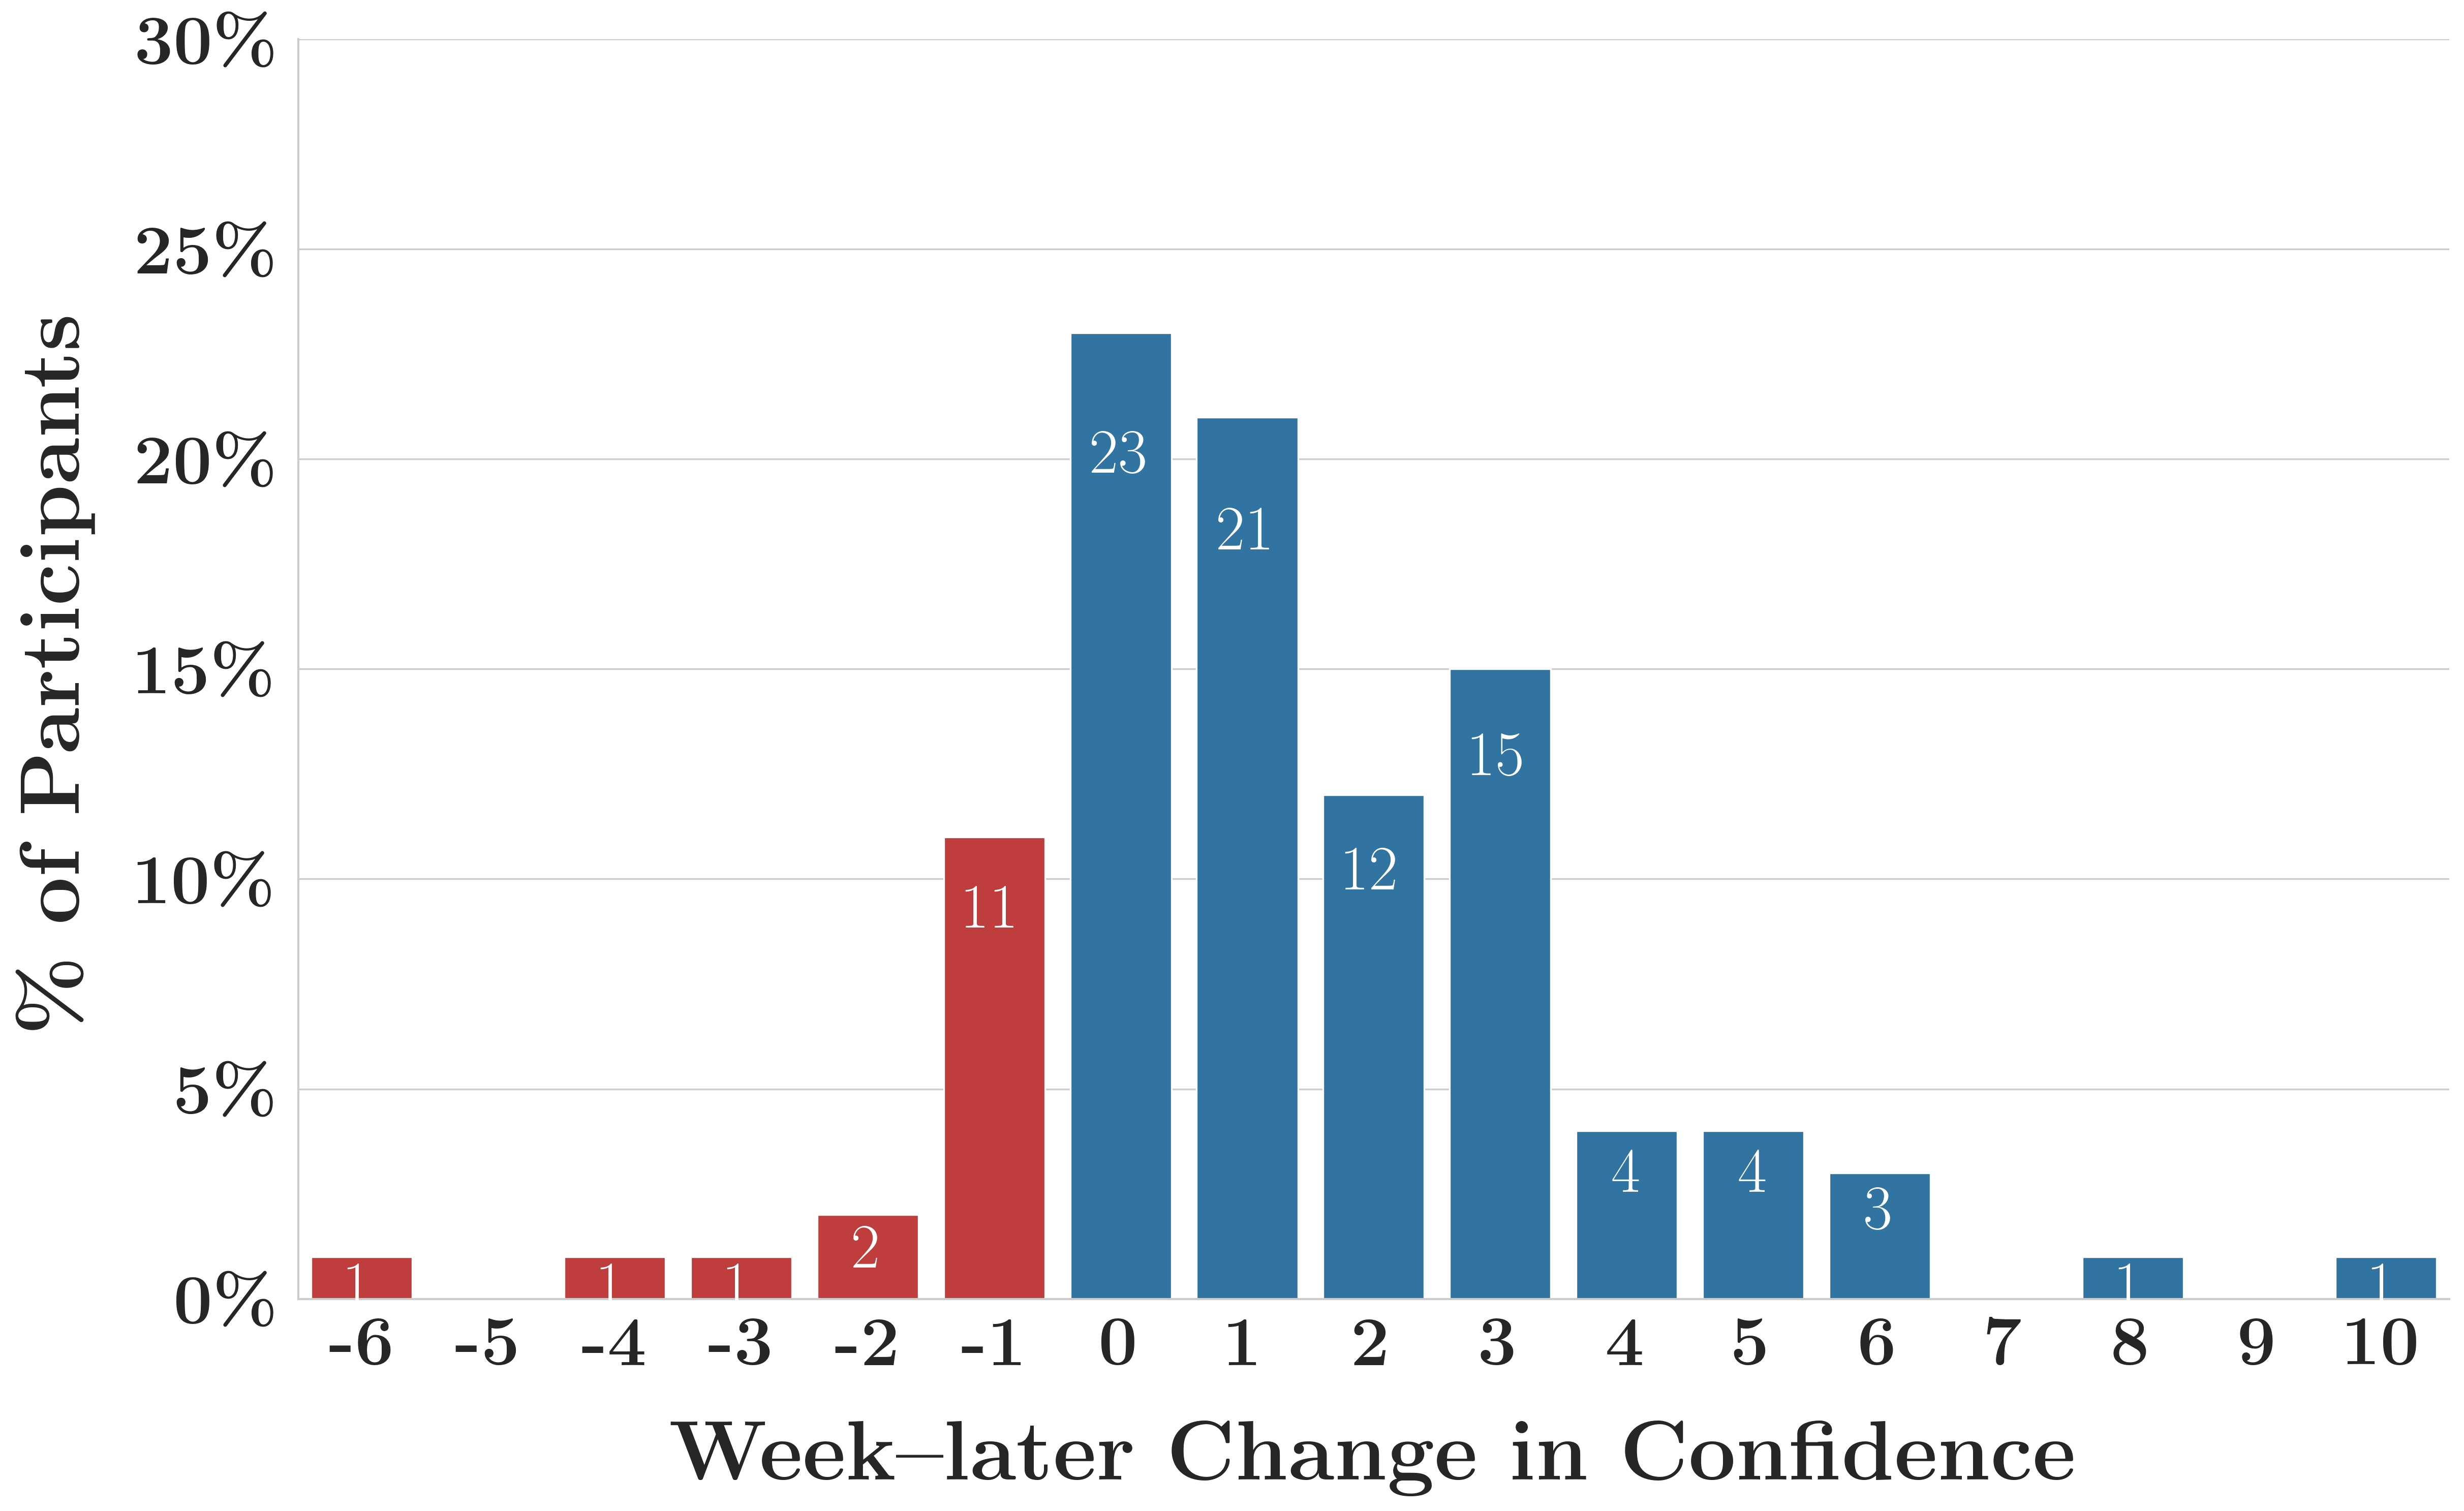
\includegraphics[width=\textwidth]{fig/MIV5.2_ruler_deltas_delta_with_week_later_keep_high_conf_False_change.png}
        \caption{MIBot v5.2}
        \label{fig:confidence_v5.2}
    \end{subfigure}
    \hfill
    \begin{subfigure}[b]{0.48\textwidth}
        \centering
        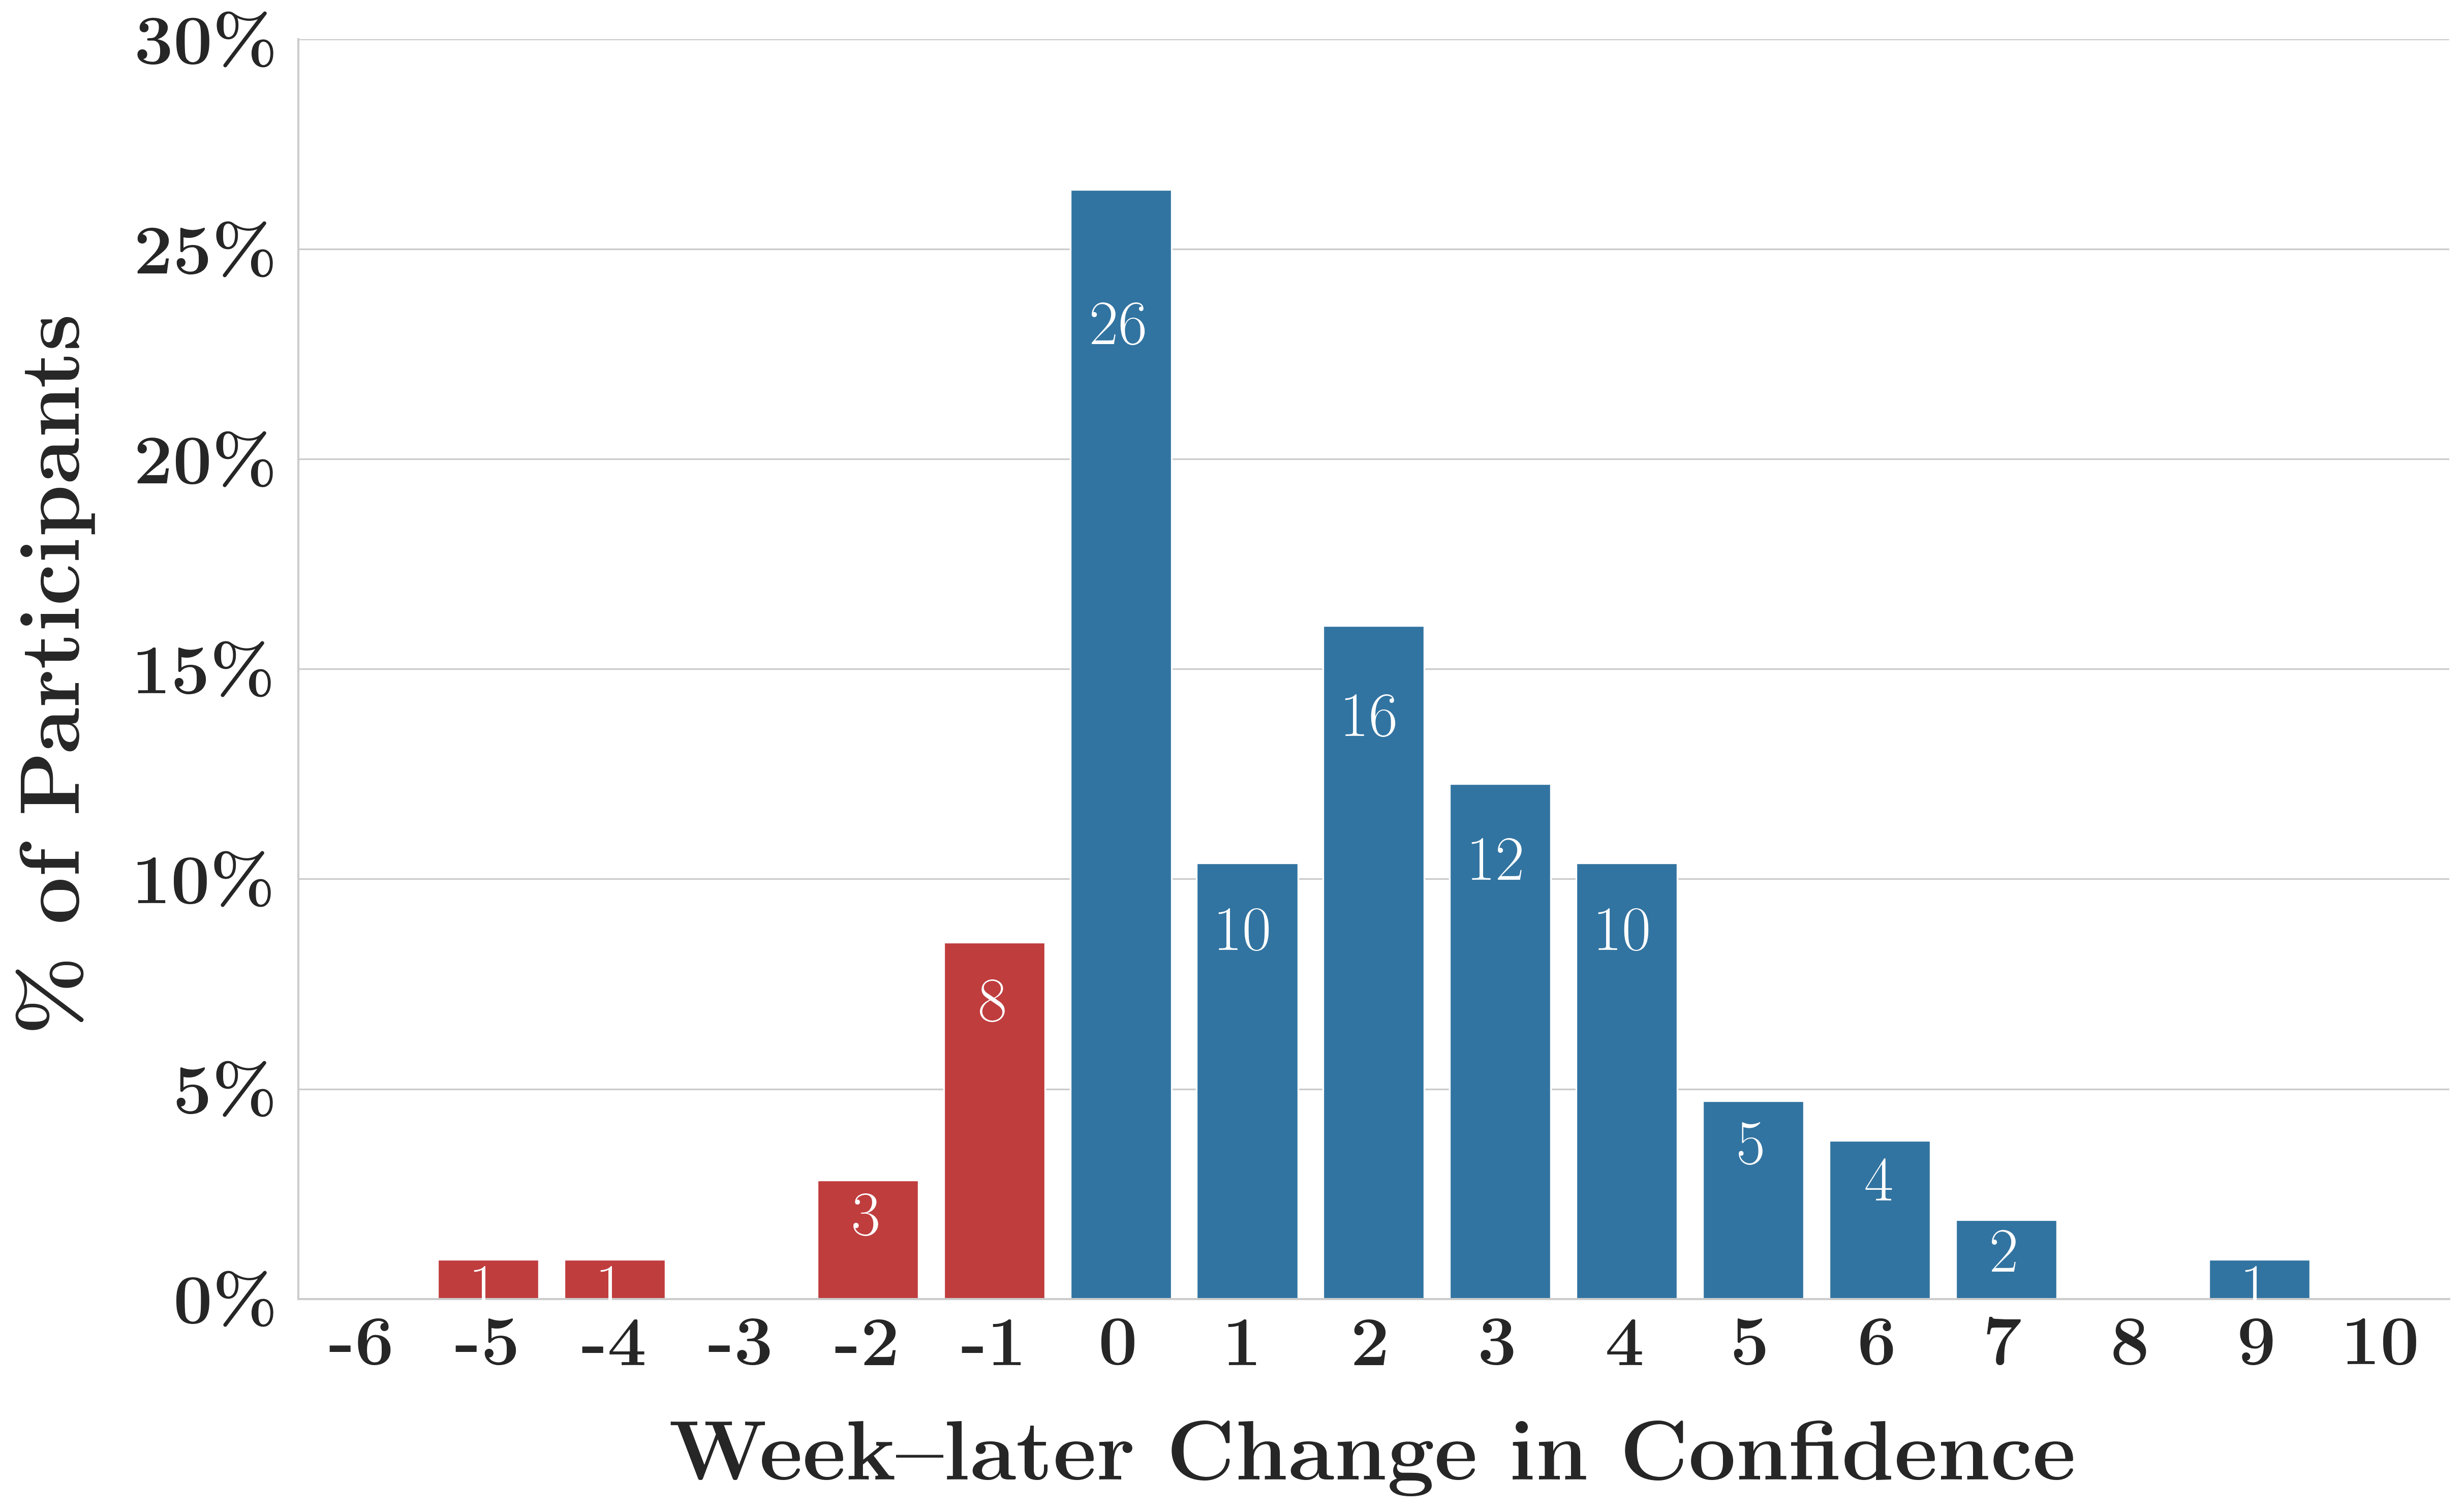
\includegraphics[width=\textwidth]{fig/2024-11-14-MIV6.3A-2024-11-22-MIV6.3A_ruler_deltas_delta_with_week_later_keep_high_conf_False_change.png}
        \caption{MIBot v6.3A}
        \label{fig:confidence_v6.3}
    \end{subfigure}

    
    \caption{Distribution of week-later confidence changes from baseline for (a) MIBot v5.2 and (b) MIBot v6.3A. Red bars indicate decreased confidence while blue bars indicate increased or unchanged confidence. MIBot v6.3A shows a higher proportion of participants with no change (26\% vs.\ 23\%) and fewer reporting decreased confidence (13\% vs.\ 16\%).}
    \label{fig:confidence_distributions}
\end{figure}










MIBot v5.2 achieved a mean confidence increase of 1.3 (SD 2.3, $p<0.001$) 
from baseline to one week later among 100 participants, and 
MIBot v6.3A achieved an increase of 1.7 (SD 2.4, $p<0.001$) among 106 participants.  
This difference was not statistically significant ($t(203.60) = 0.98$, 
$p = 0.165$, one-tailed, Cohen's $d = 0.14$). As shown in Figure~\ref{fig:confidence_distributions}, 
the distribution of confidence changes reveals interesting patterns: MIBot v6.3A 
resulted in more participants maintaining their baseline confidence (28\% vs.\ 23\% 
with no change) and fewer experiencing decreased confidence (13\% vs.\ 17\%).

For importance to quit, MIBot v5.2 achieved a significant increase of 0.7 (SD 2.0, $p<0.001$), while MIBot v6.3A showed a more modest but still significant gain of 0.5 (SD 1.7, $p<0.005$). Readiness changes were minimal and non-significant for both versions (v5.2: 0.4, SD 1.7, $p=0.01$; v6.3A: 0.3, SD 2.4, $p=0.22$).

\subsection{Perceived Empathy Comparisons}

\begin{figure}[htbp]
    \centering
    \begin{subfigure}[b]{0.48\textwidth}
        \centering
        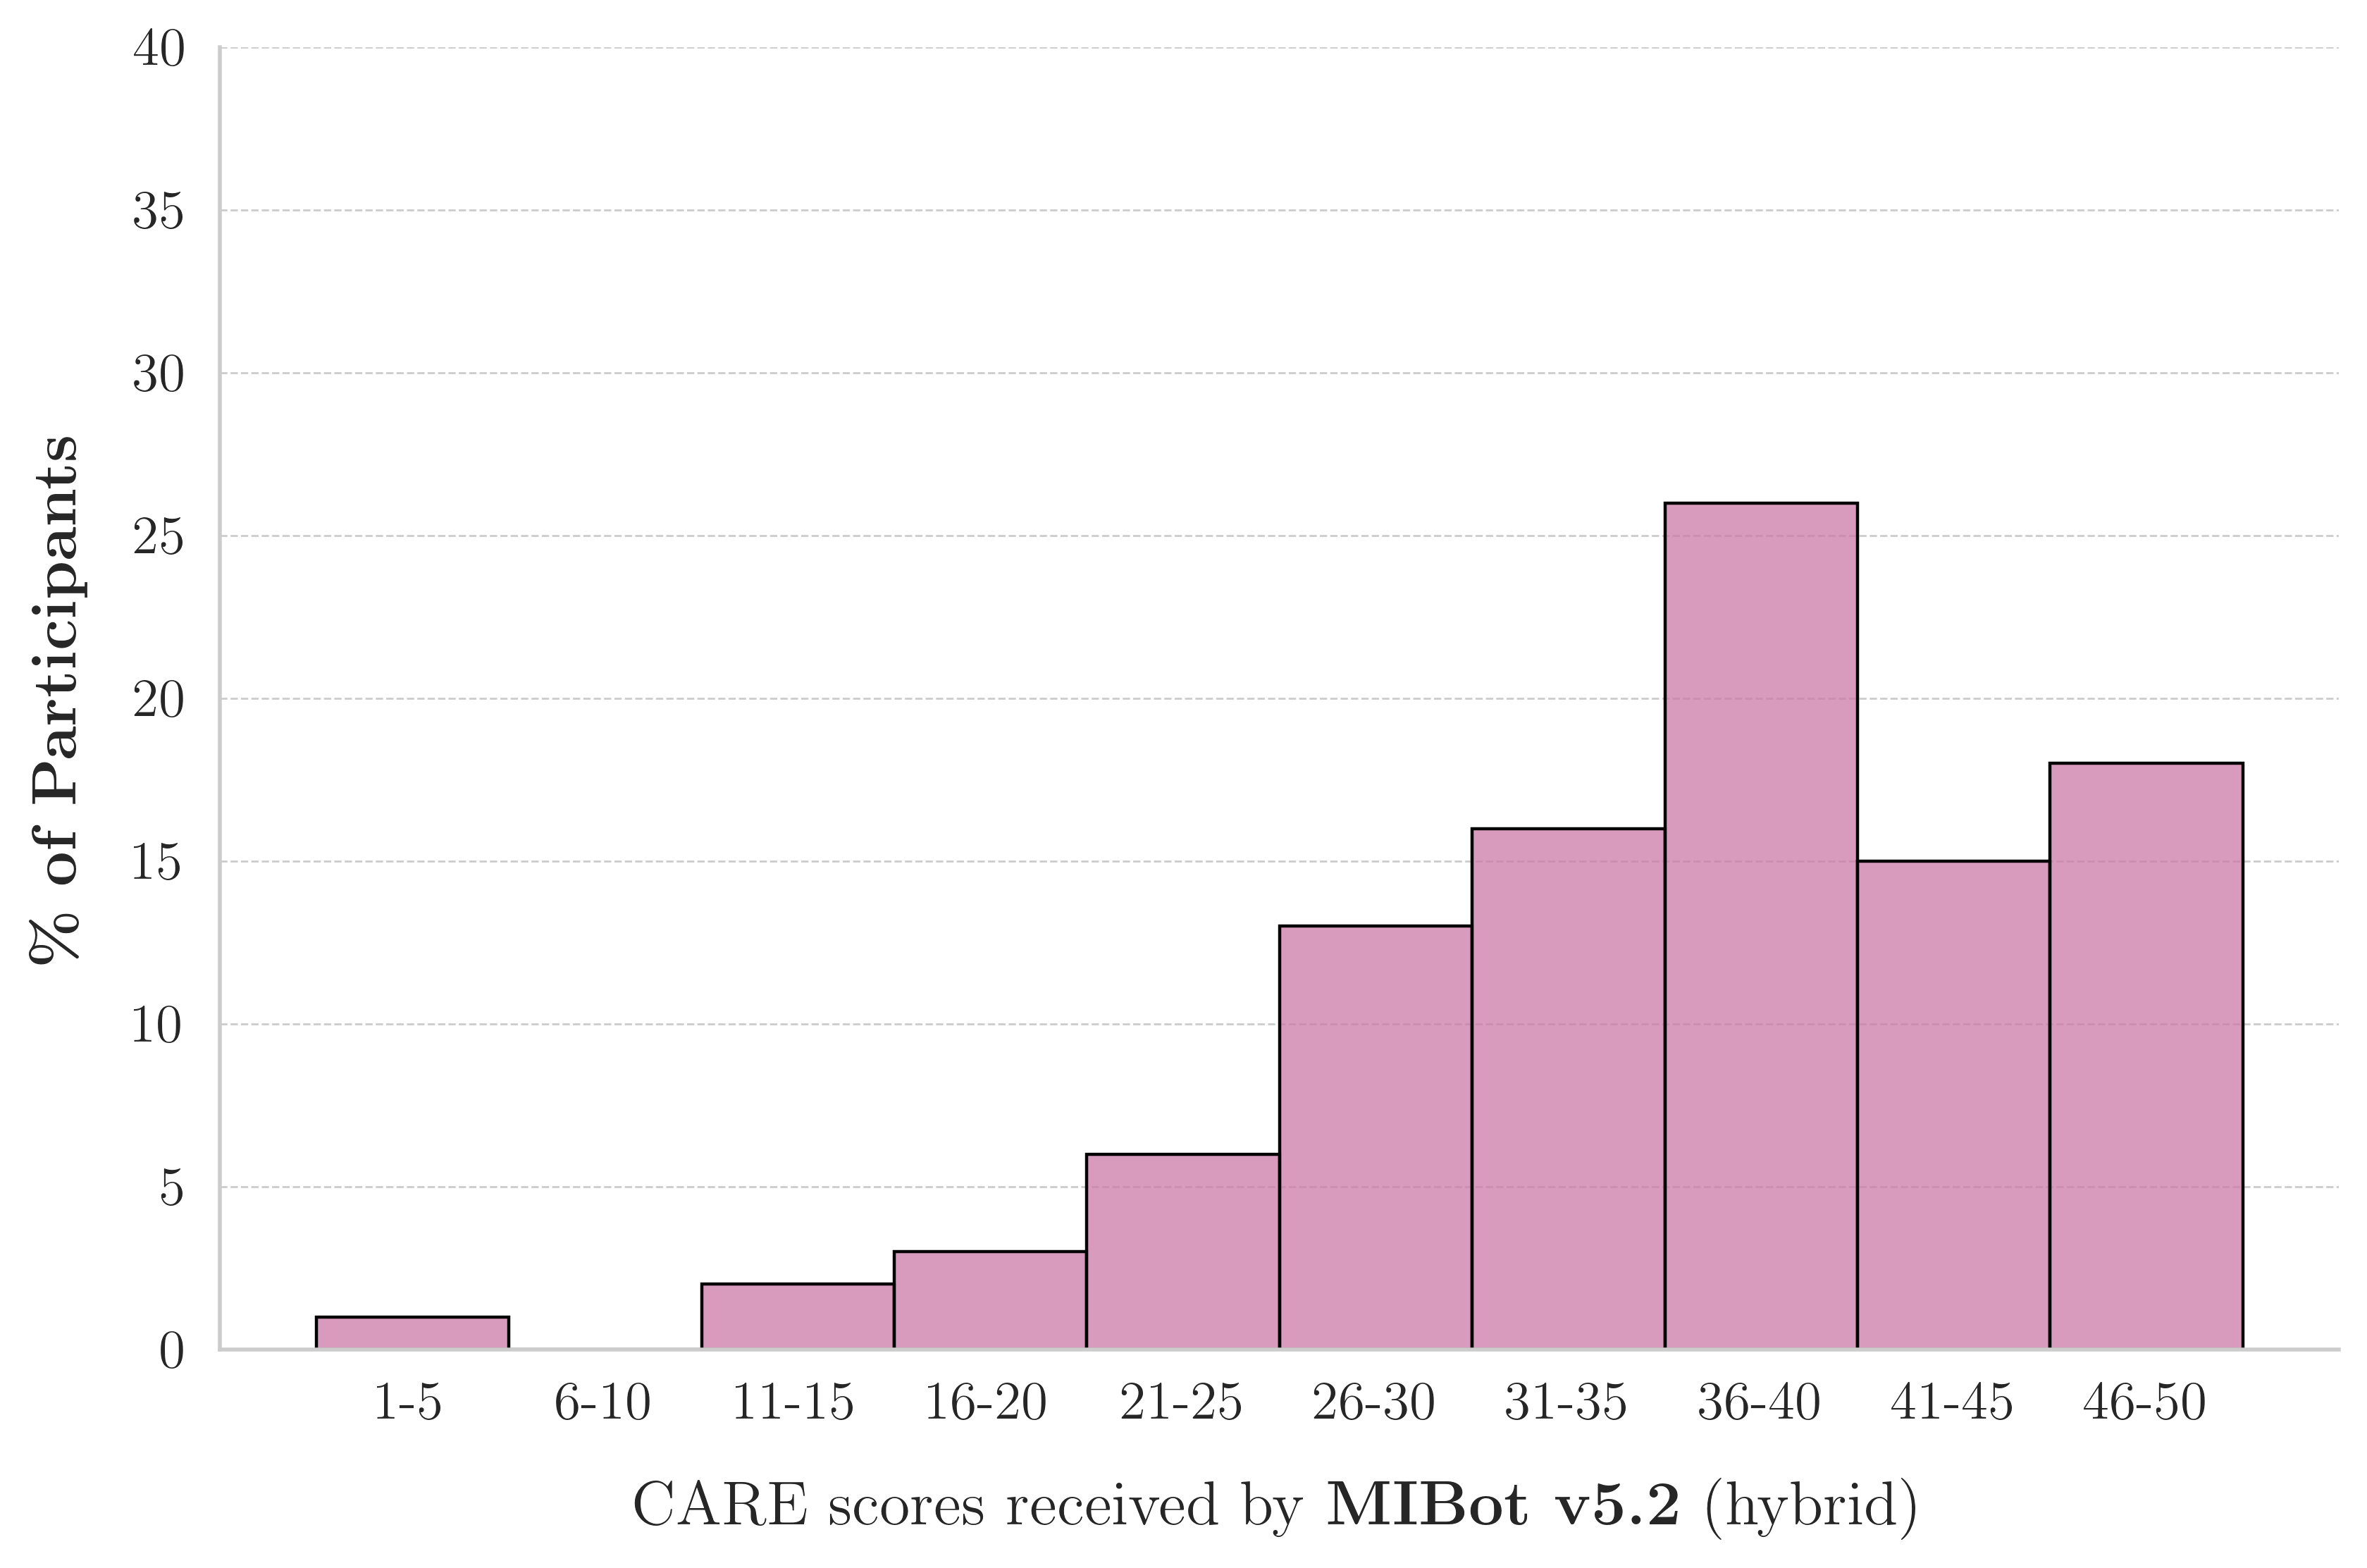
\includegraphics[width=\textwidth]{fig/MIV5.2_care_scores_histogram.png}
        \caption{MIBot v5.2 (hybrid)}
        \label{fig:care_v5.2}
    \end{subfigure}
    \hfill
    \begin{subfigure}[b]{0.48\textwidth}
        \centering
        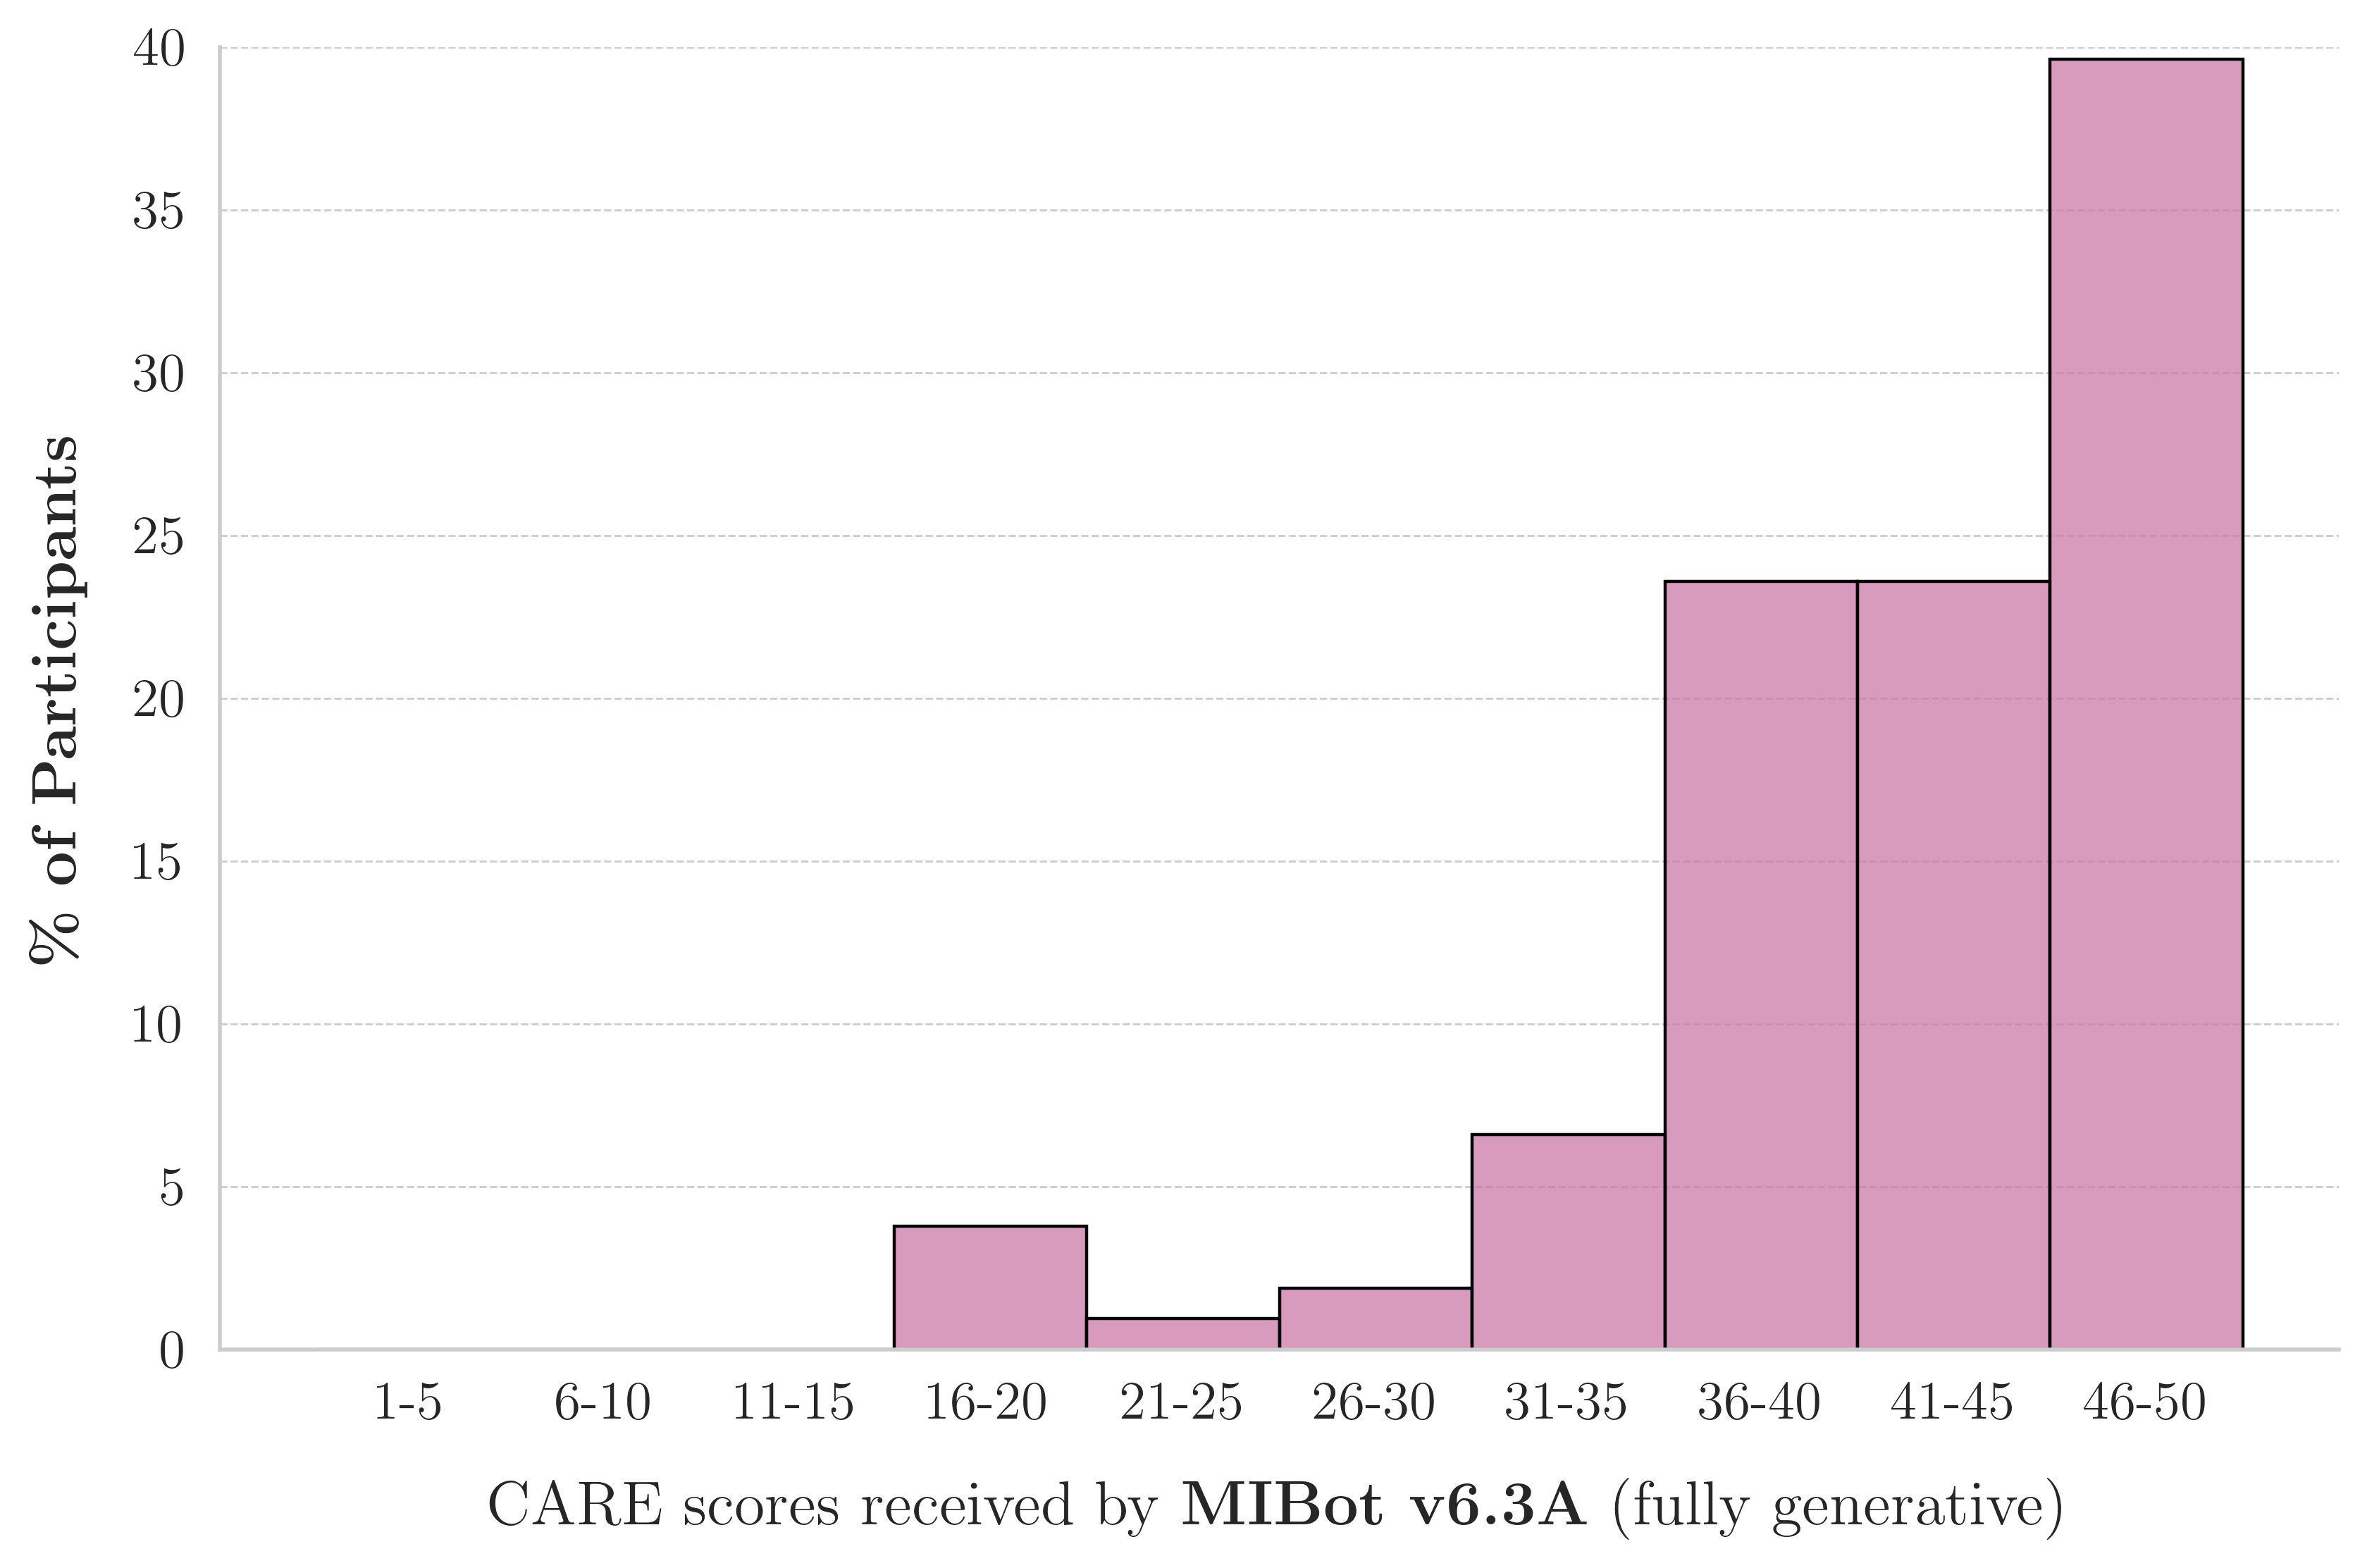
\includegraphics[width=\textwidth]{fig/2024-11-14-MIV6.3A-2024-11-22-MIV6.3A_care_scores_histogram.png}
        \caption{MIBot v6.3A (fully generative)}
        \label{fig:care_v6.3}
    \end{subfigure}
    \caption{Distribution of CARE empathy scores for (a) MIBot v5.2 and (b) MIBot v6.3A. The fully generative v6.3A shows a pronounced rightward shift with $\sim$40\% of participants scoring in the highest range (46--50) compared to only $\sim$18\% for the hybrid v5.2. Lower scores (below 30) were nearly eliminated in v6.3A.}
    \label{fig:care_distributions}
\end{figure}

\begin{figure}[htbp]
    \centering
    \includegraphics[width=0.98\textwidth]{fig/combined_care_scores_with_improvement.png}
    \caption{Question-wise mean CARE scores comparing MIBot v5.2 (hybrid) and v6.3A (fully generative). The fully generative version shows consistent improvements across all dimensions of empathy. Bars displayed in ascending order of relative improvement.}
    \label{fig:care_questions}
\end{figure}

 MIBot v5.2 achieved a mean CARE score of 36 ($SD = 9.1$), with only 3\% of participants awarding perfect score, while MIBot v6.3A achieved a mean score of 42 ($SD = 7.5$), with 11\% receiving perfect scores. This difference was statistically significant ($t(191.67) = 4.96$, $p < .001$, Cohen's $d = 0.70$), representing a medium-to-large effect size, and suggests that the fully-generative  responses of v6.3A significantly improved perceived empathy. Figure~\ref{fig:care_distributions} illustrates the distributional shift between versions. The hybrid v5.2 shows a relatively normal distribution centred in the mid-30s range, with considerable spread across all score ranges, whereas v6.3A demonstrates a clear rightward skew, with 40\% of participants rating the chatbot in the highest range (46--50).

To understand which aspects of empathetic interaction improved most, Figure~\ref{fig:care_questions} presents the mean scores across all ten CARE dimensions. The fully generative approach exhibits improvements across every dimension, with particularly notable gains in emotional and communicative aspects. The largest relative improvement was observed in ``showing care and compassion'' (+32\%), reflecting the chatbot's enhanced ability to maintain an encouraging tone. Interestingly, the dimension of ``making a plan of action with you'' remained the weakest aspect for both versions (2.73 for v5.2, 3.59 for v6.3A), despite showing considerable relative improvement (+32\%). It is worth noting that MIBot v6.3 was prompted with detailed guidelines on how to make a plan of action with the client. Despite this, planning seems to be one of its weak areas.



\subsection{Implications of the Comparison}

The fully generative MIBot v6.3A chatbot scores higher on CARE, the measure of perceived therapeutic alliance. This improvement suggests that participants experienced more authentic, personalized interactions when the entire conversation --- not just reflections --- emerged from the language model's contextual understanding. However, both the chatbots scored the same on our primary metric of effectiveness, viz., the week-later change in confidence, indicating that the core therapeutic mechanism of MI may be responsible for most of the gains in confidence. This finding aligns with prior work showing that even simple question-asking can produce substantial benefits \citep{brown2023mi}, though the enhanced empathy of full generation may improve engagement and retention in real-world deployment.

\section{AutoMISC Analysis}
\label{sec:mi-adherence}

To evaluate the chatbot's adherence to MI principles, we analyzed counsellor and client utterances from the feasibility study transcripts (Section~\ref{sec:feasability}) using \margindex{AutoMISC}AutoMISC, an automated annotation system originally described in \citet{mahmood-etal-2025-fully}\footnote{A comprehensive description of the AutoMISC system by \citet{ali2025automated} is forthcoming}.
The system assigns behavioural codes to each utterance: counsellor utterances are classified as MI-Consistent (MICO), MI-Inconsistent (MIIN), Reflection (R), Question (Q), or Other (O), while client utterances are categorized as change talk (C), sustain talk (S), or neutral (N). Following annotation of all utterances, we computed per-transcript summary metrics to quantify MI adherence. These comprise:

\begin{itemize}

    \item \textbf{\margindex{Percentage MI-Consistent Responses (\%MIC)}Percentage MI-Consistent Responses (\%MIC):} The proportion of counsellor utterances that align with MI principles. Higher values indicate greater adherence to MI methodology.
    
    \item \textbf{\margindex{Reflection-to-Question Ratio (R:Q)}[R:Q]Reflection-to-Question Ratio (R:Q):} The ratio of counsellor utterances labelled as reflection (R) to those labelled as question (Q). This metric assesses the balance between reflective listening and questioning. Values between 1 and 2 are considered indicative of proficiency \citep{moyers2016miti}.

    \item \textbf{\margindex{Percentage Change Talk (\%CT)}Percentage Change Talk (\%CT):} The proportion of client utterances expressing motivation toward behaviour change. Higher values are associated with improved behavioural outcomes \citep{apodaca2009}.

\end{itemize}

\subsection{Contextualizing AutoMISC metrics with the HLQC Dataset}
To provide a point of comparison for the MISC summary metrics, we also ran AutoMISC on the HighLowQualityCounselling (HLQC) dataset  \cite{perez-rosas-etal-2019-makes}, a publicly available\footnote{ \url{https://lit.eecs.umich.edu/downloads.html}} corpus of transcribed MI counselling demonstrations. The HLQC dataset comprises 155 high-quality (HLQC\_\textbf{HI}) and 104 low-quality (HLQC\_\textbf{LO}) transcripts sourced from public websites.
We computed summary scores separately for these subsets and then compared MIBot's summary metrics against those of both HLQC\_HI and HLQC\_LO.

\subsection{Counsellor Behaviour Metrics}
Table~\ref{table:automisc_summary} summarizes the counsellor-specific AutoMISC summary metrics across the 106 transcripts. The mean percentage of MI-consistent responses (\%MIC) was 98 (SD 3.6), higher than the high-quality counsellor sessions in the HLQC dataset (92, SD 9.8). MIBot's reflection-to-question ratio (R:Q) was 1.3 (SD 0.3), comfortably within the 1--2 range recommended for human practitioners \cite{moyers2016miti}.

\begin{table}[ht]
  \centering
  \small
  \setlength{\tabcolsep}{4pt}
  \renewcommand{\arraystretch}{1.1}
  \begin{tabular}{@{}lcc@{}}
    \toprule
    \textbf{Metric} & \textbf{MIBot} & \textbf{HLQC\_HI (high-quality)} \\
    \midrule
    \%MI-consistent (\%MIC) & 98 (3.6) & 92 (9.8) \\
    Reflection-to-Question Ratio (R:Q) & 1.3 (0.3) & 2.3 (5.7) \\
    \bottomrule
  \end{tabular}
  \caption{AutoMISC counsellor-specific summary metrics for MIBot compared to high-quality human counselling sessions. Values shown as mean (standard deviation).}
  \label{table:automisc_summary}
\end{table}

Figure~\ref{fig:misc_distributions} shows violin plots comparing the distribution of \%MIC, R:Q, and \%CT across MIBot conversations with the HLQC benchmarks. The \%MIC scores are tightly clustered near 100\%, with only a few transcripts falling below 80\%. The R:Q distribution is centred around 1.3, showing less variance than human counsellors who range from pure question-asking (R:Q near 0) to heavy reflection use (R:Q $>$ 5).

\begin{figure}[ht]
  \centering
  \begin{subfigure}[b]{0.32\textwidth}
    \centering
    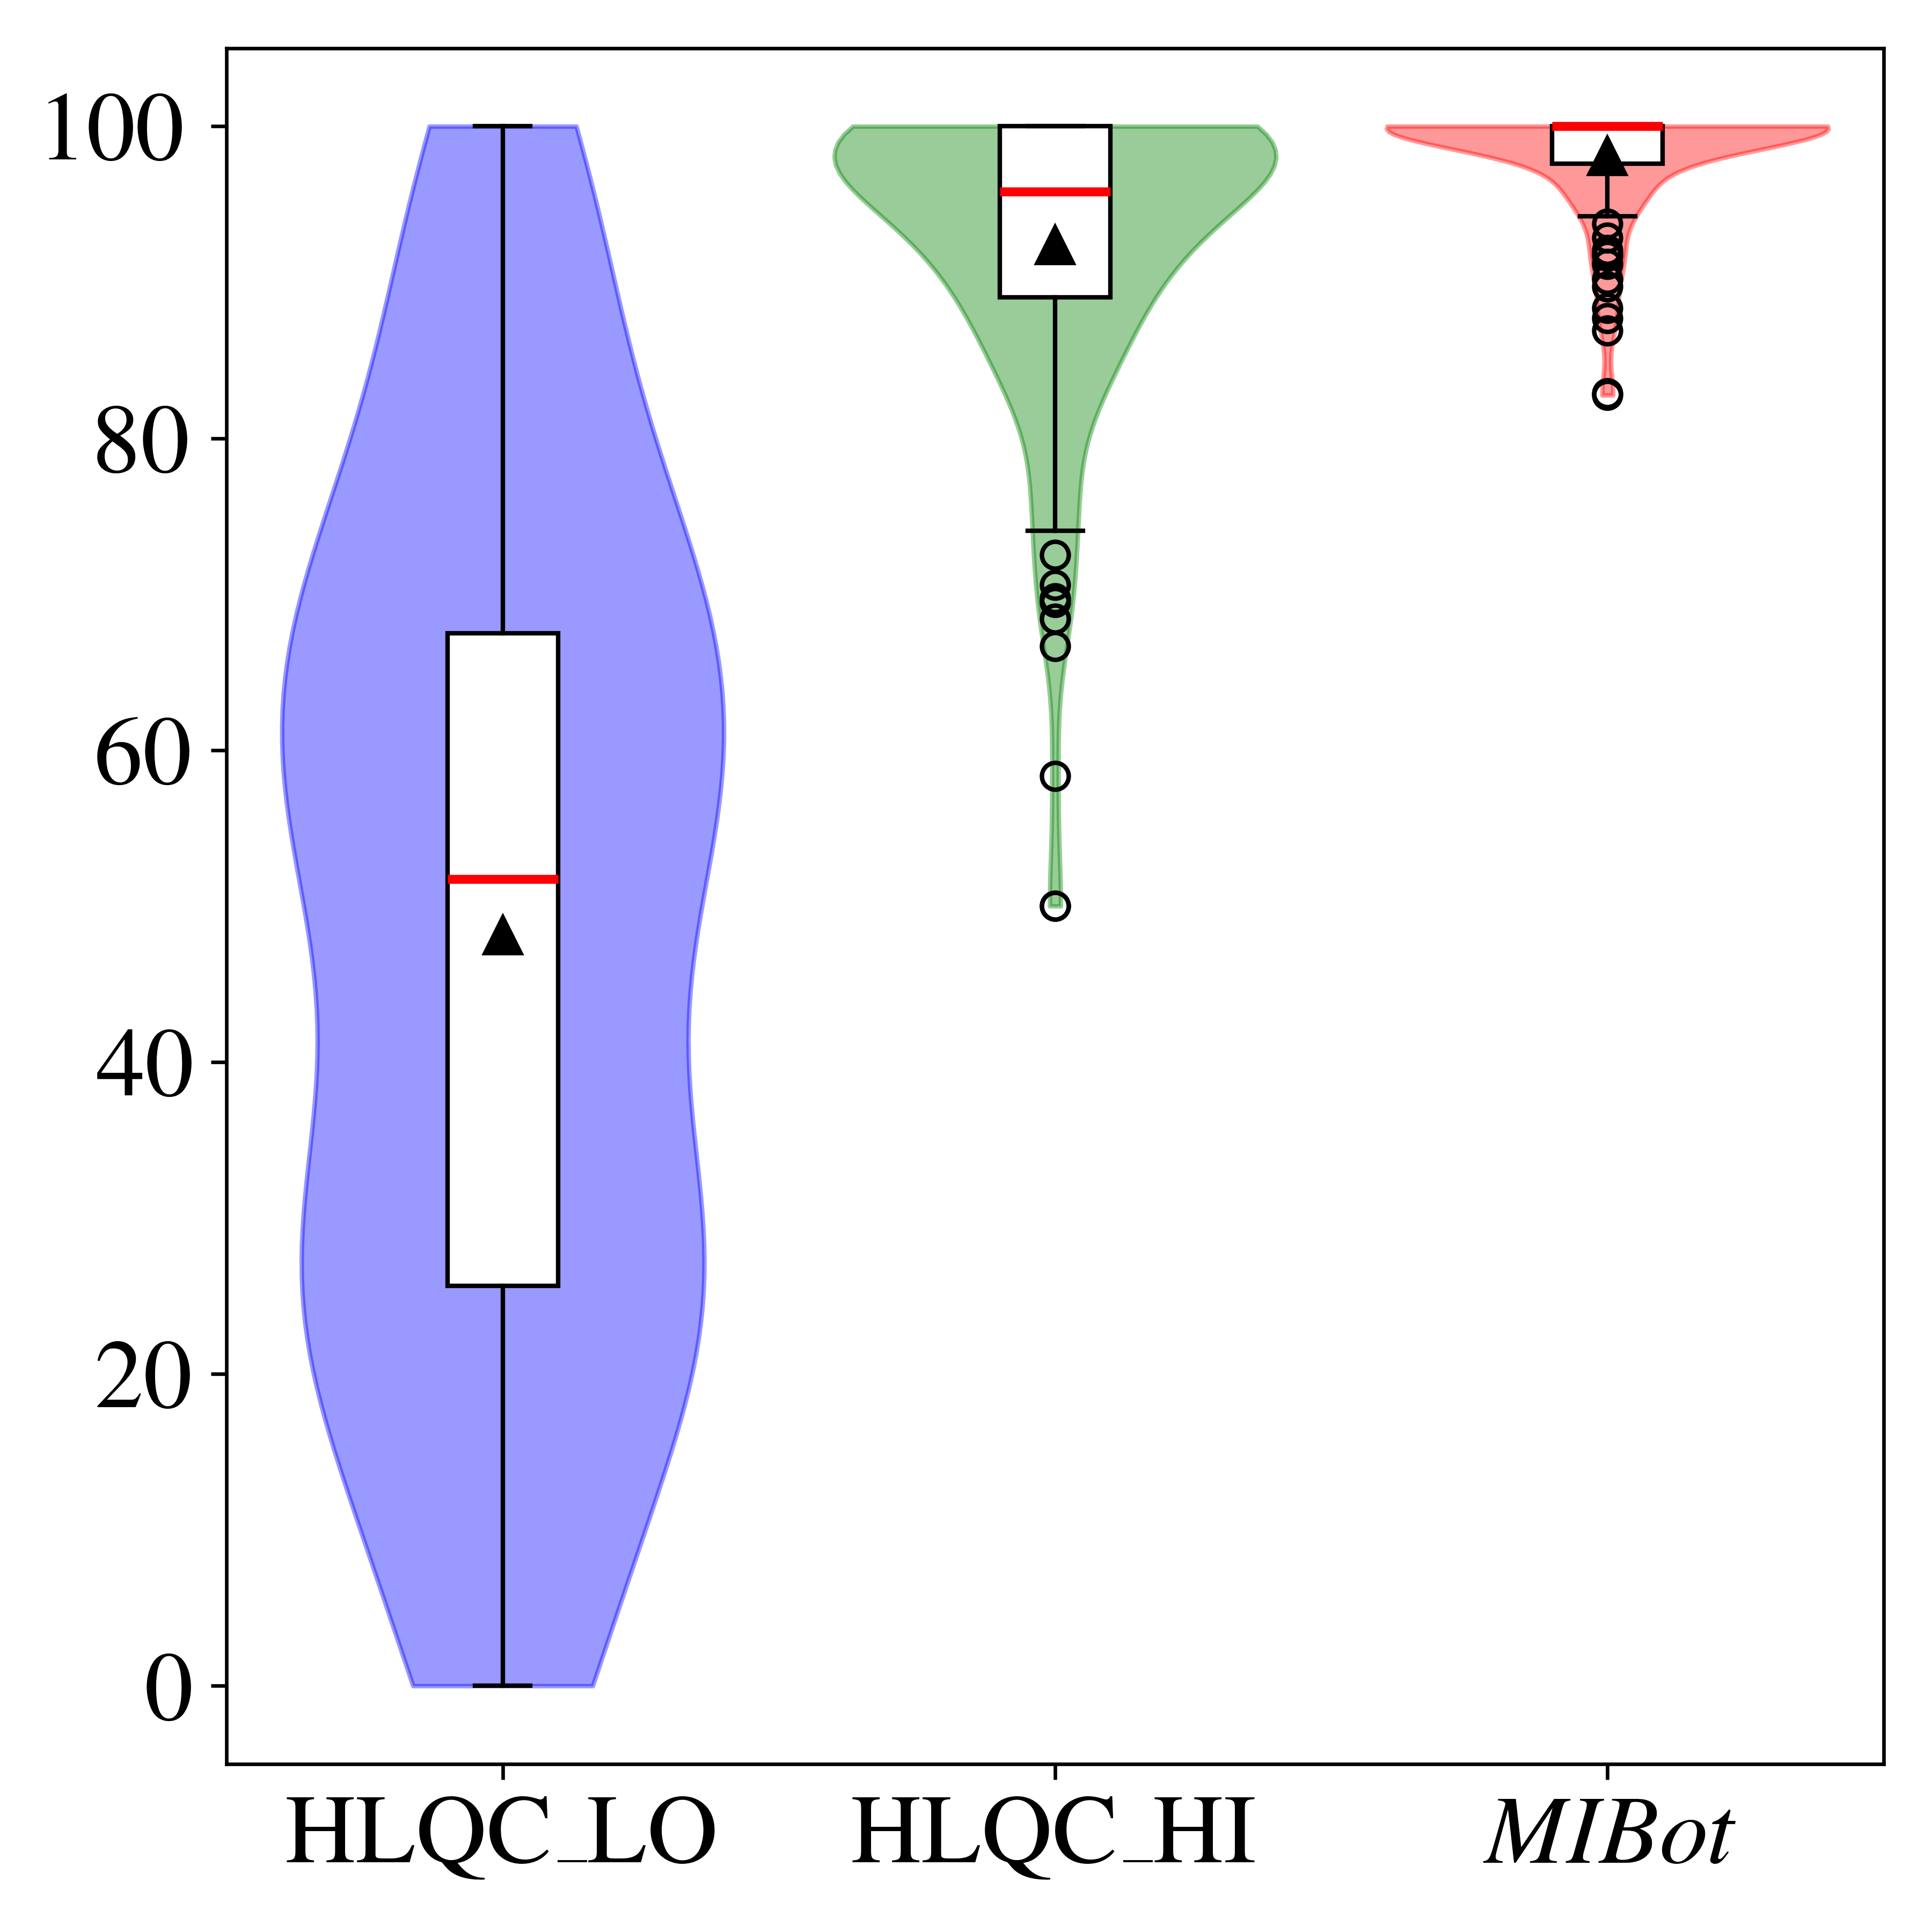
\includegraphics[width=\textwidth]{fig/mic.png}
    \caption{\%MIC}
  \end{subfigure}
  \hfill
  \begin{subfigure}[b]{0.32\textwidth}
    \centering
    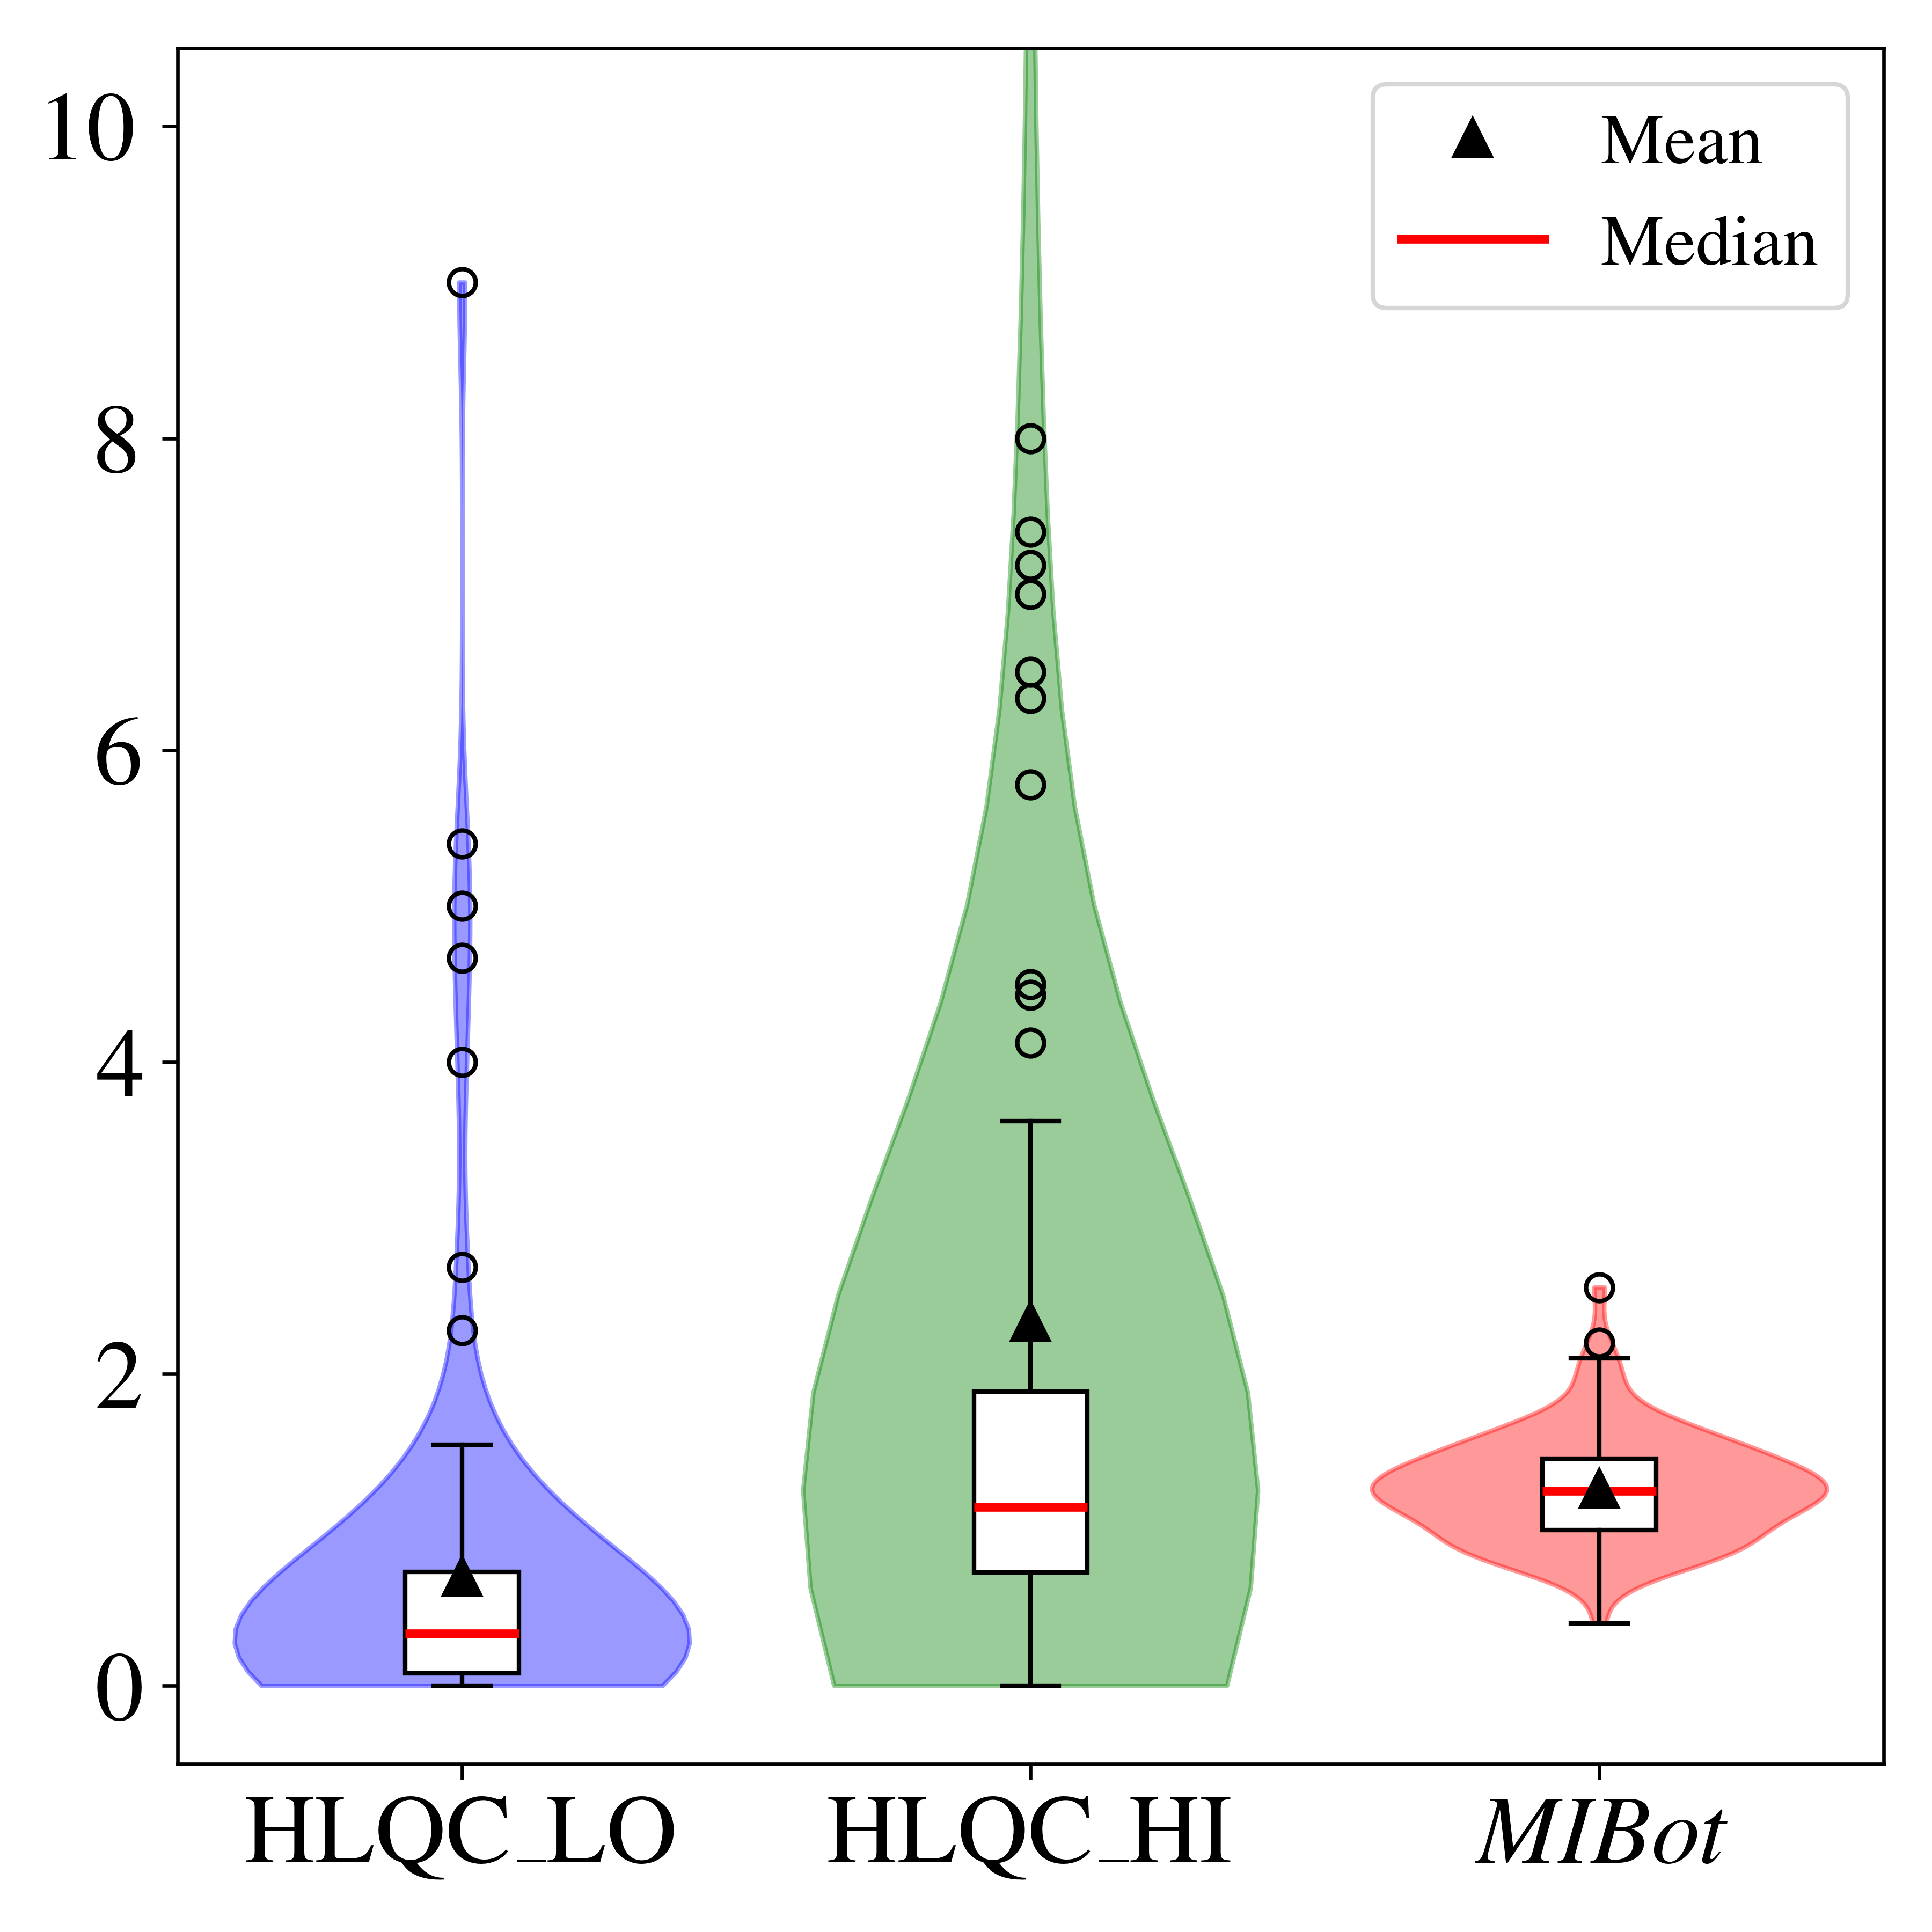
\includegraphics[width=\textwidth]{fig/rq.png}
    \caption{R:Q}
  \end{subfigure}
  \hfill
  \begin{subfigure}[b]{0.32\textwidth}
    \centering
    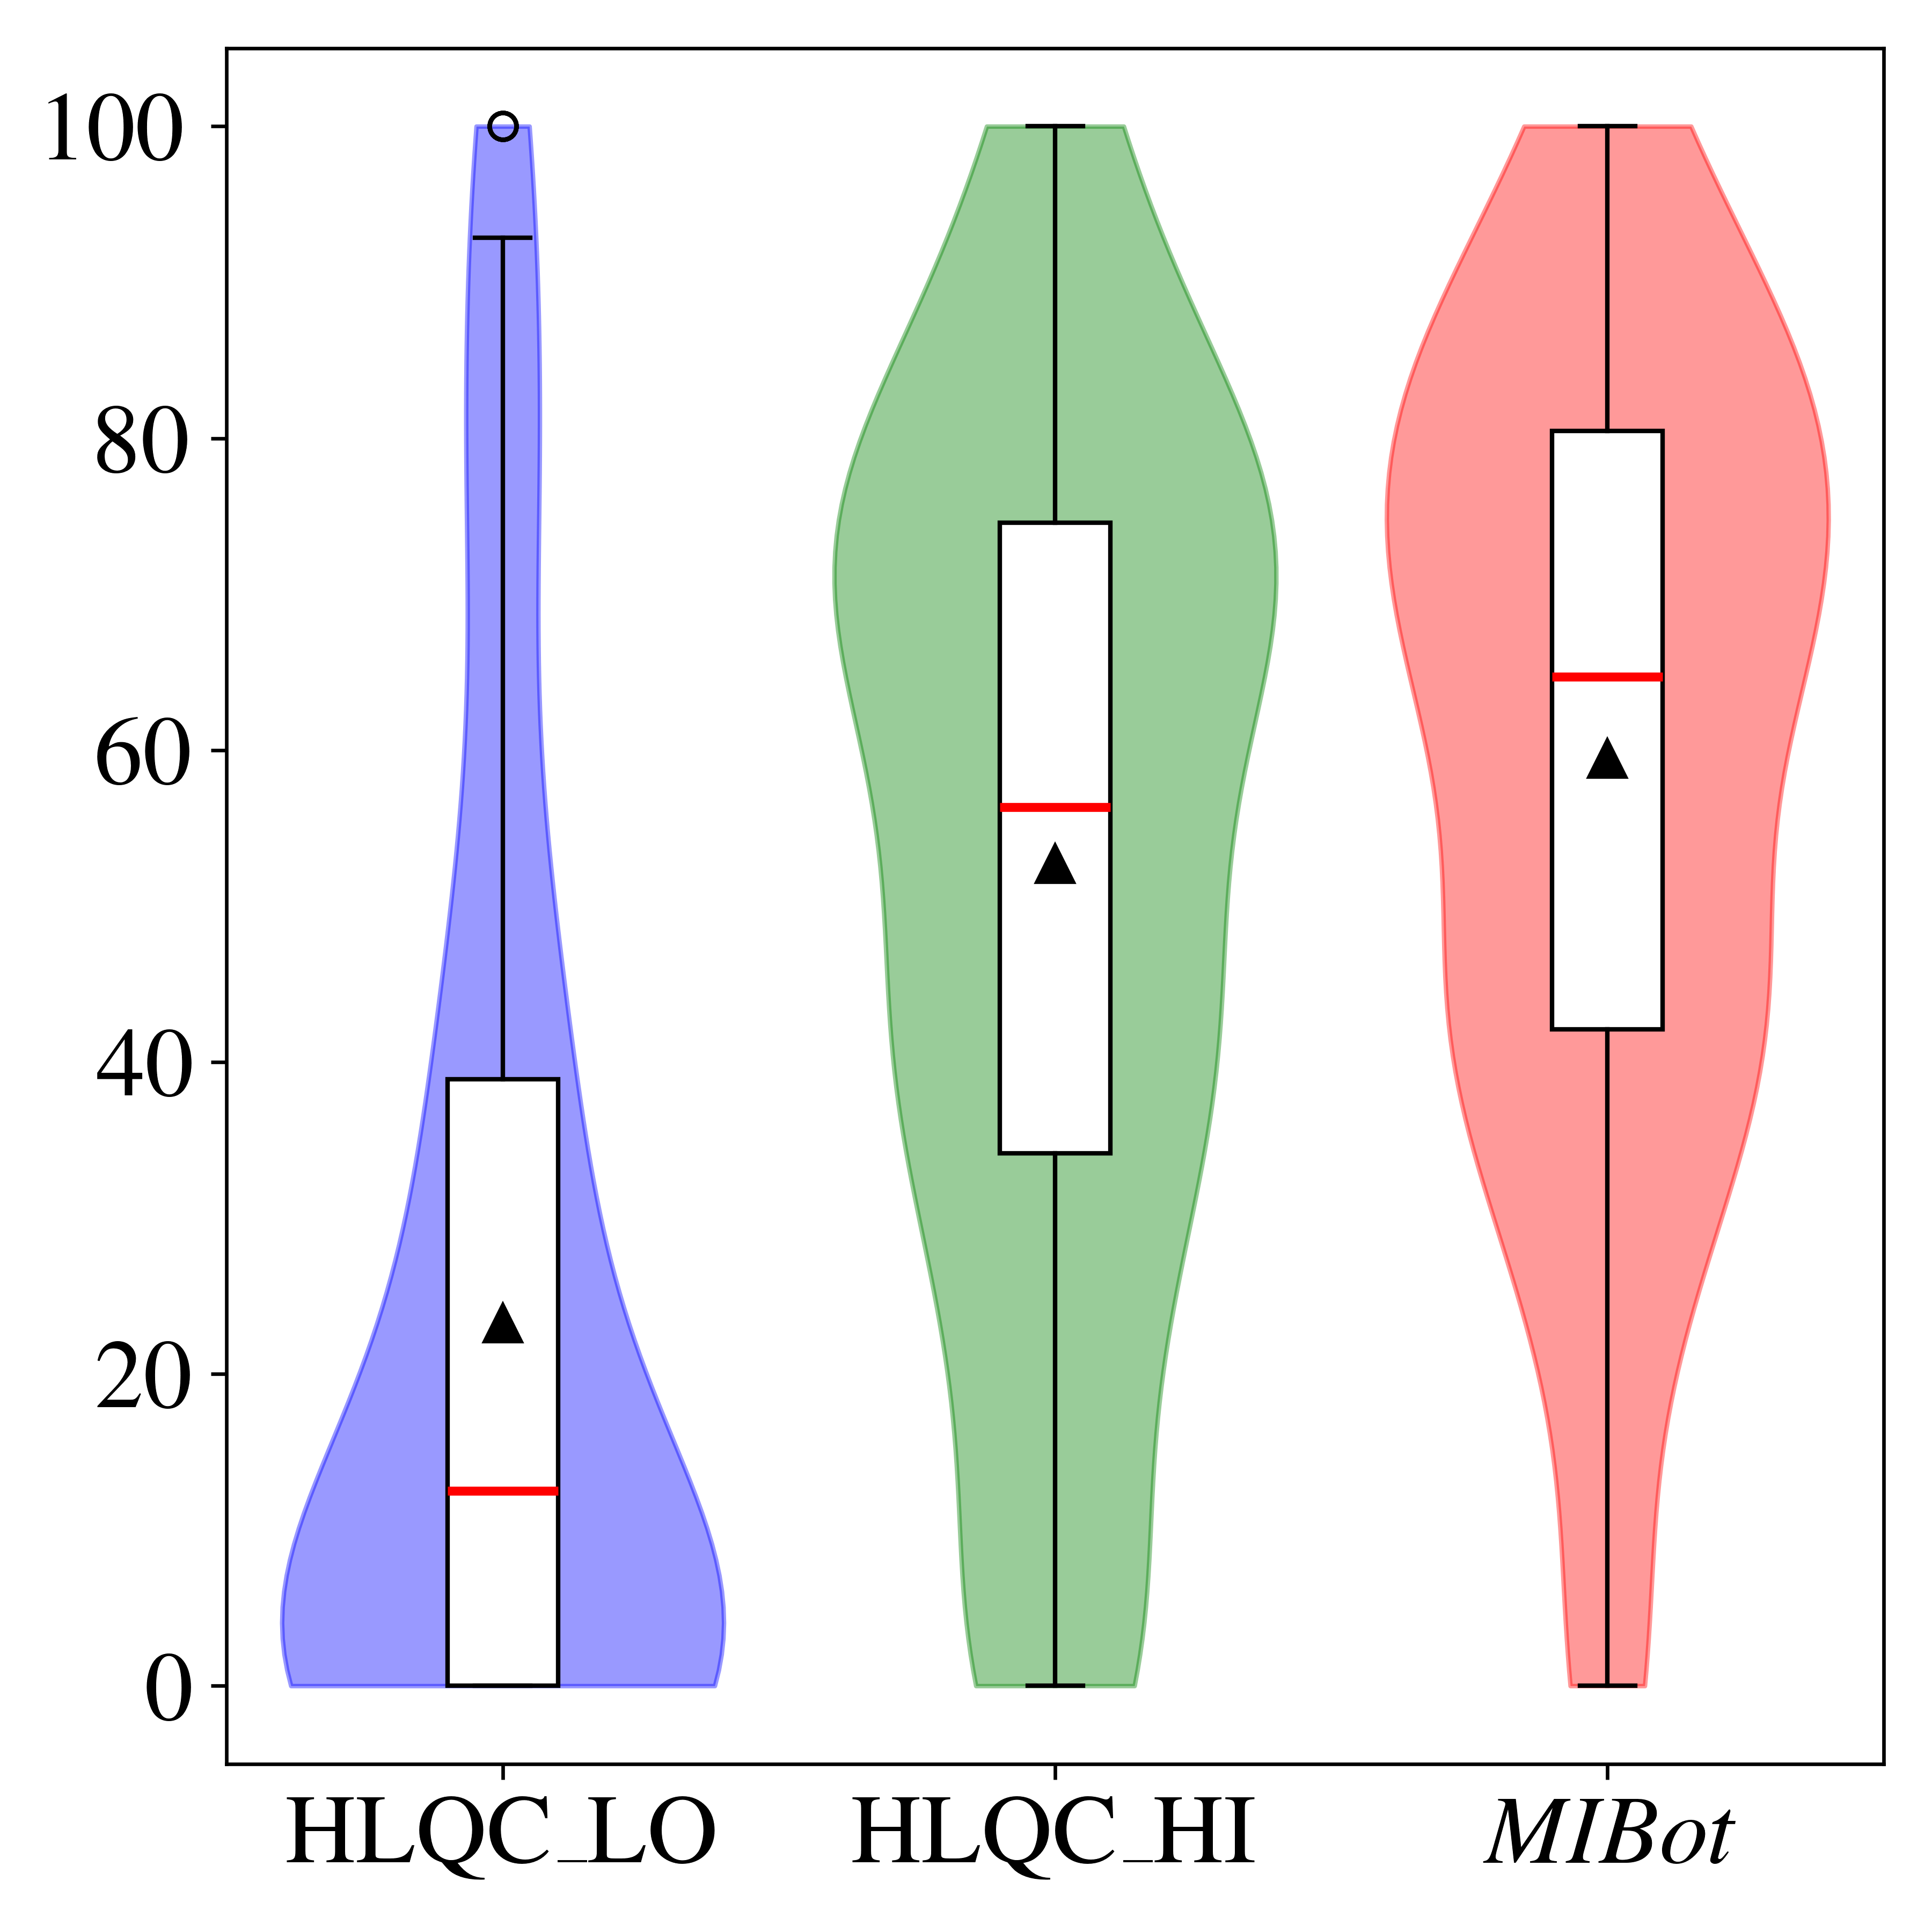
\includegraphics[width=\textwidth]{fig/ct.png}
    \caption{\%CT}
  \end{subfigure}
  \caption{Comparison of MISC summary score distributions across datasets. (a) Percentage MI-Consistent Responses (\%MIC), (b) Reflection to Question Ratio (R:Q), (c) Percentage Client Change Talk (\%CT).}
  \label{fig:misc_distributions}
\end{figure}


\subsection{Client Change Talk Analysis}



\begin{table}[ht]
  \centering
  \small
  \setlength{\tabcolsep}{4pt}
  \renewcommand{\arraystretch}{1.1}
  \begin{tabular}{@{}lcc@{}}
    \toprule
    \textbf{Metric} & \textbf{MIBot} & \textbf{HLQC\_HI (high-quality)} \\
    \midrule
    \%Change Talk (\%CT) & 59 (29.6) & 53 (28.54) \\
    \bottomrule
  \end{tabular}
  \caption{AutoMISC client-specific summary metric for MIBot compared to high-quality human counselling sessions. Values shown as mean (standard deviation).}
  \label{table:automisc_summary_client}
\end{table}


Figure~\ref{fig:misc_distributions} c illustrates the distribution of \%CT across conversations. Most sessions by MIBot a \%CT of $>$ 60\% and the distribution closely matches that of \textbf{HLQC\_HI} dataset.Overall, the mean \%CT was 59\% for MIBot as compared to 53\% for \textbf{HLQC\_HI} dataset.


%%%%%%%%%%%%%%%%%%%%%%%%%%%%%%%%%%%%%%%%%%%%%%%%

% WIP Below

% Please edit it later!


%%%%%%%%%%%%%%%%%%%%%%%%%%%%%%%%%%%%%%%%%%%%%%%%%




























\section{Behavioural Outcomes}


\label{sec:behavioural-outcomes}

\subsection{Quit Attempts at One Week}

Table~\ref{table:quit_attempts} summarises quit attempt behaviour before and after the MIBot conversation. Prior to the conversation, 32.1\% (34/106) of participants had made a quit attempt in the previous week. At the one-week follow-up, 34.9\% (37/106) reported making a quit attempt since the conversation. Crucially, among the 72 participants who had not attempted to quit before the conversation, 15 (20.8\%) made their first attempt following the MIBot session.

\begin{table}[ht]
  \centering
  \small
  \setlength{\tabcolsep}{4pt}
  \renewcommand{\arraystretch}{1.1}
  \begin{tabular}{@{}lcc@{}}
    \toprule
    \textbf{Quit Attempt Status} & \textbf{Pre-conversation} & \textbf{Post-conversation} \\
    \midrule
    Made attempt & 34 (32.1\%) & 37 (34.9\%) \\
    No attempt & 72 (67.9\%) & 69 (65.1\%) \\
    \midrule
    New attempters & -- & 15 (14.2\%) \\
    Sustained attempters & -- & 22 (20.8\%) \\
    \bottomrule
  \end{tabular}
  \caption{Quit attempt behaviour before and after MIBot conversation.}
  \label{table:quit_attempts}
\end{table}

Participants who made quit attempts post-conversation showed larger confidence gains (mean +2.43) compared to those who did not attempt (+1.35, $p<0.05$). This bidirectional relationship---where confidence predicts attempts and attempts reinforce confidence---aligns with social cognitive theory \citep{Bandura1986}.

\subsection{Self-Reported Behavioural Changes}

Beyond formal quit attempts, participants reported various \margindex{Harm Reduction Behaviours}harm reduction behaviours. Analysis of open-ended responses revealed five main categories of behavioural change:

\begin{enumerate}
\item \textbf{Reduced consumption} (42\% of participants): ``Cut down from 20 to 12 cigarettes a day''
\item \textbf{Delayed first cigarette} (28\%): ``Now waiting until after breakfast instead of immediately upon waking''
\item \textbf{Substitution strategies} (31\%): ``Using nicotine gum when cravings hit at work''
\item \textbf{Environmental changes} (19\%): ``Removed ashtrays from the house and car''
\item \textbf{Social support seeking} (23\%): ``Told my partner about wanting to quit and asked for support''
\end{enumerate}

These incremental changes, while not constituting complete cessation, represent important steps in the behaviour change process and align with harm reduction approaches increasingly recognised in tobacco control \citep{Abrams2018}.

\section{Conversation Analysis}
\label{sec:conversation-analysis}

\subsection{Quantitative Dynamics}

Conversations ranged from 36 to 163 utterances (median 78, mean 80.7, SD 29.4), with counsellor utterances comprising 55\% of the total. The median conversation lasted approximately 19 minutes based on participant self-report. Table~\ref{table:conversation_metrics} summarizes key quantitative metrics.

\begin{table}[ht]
  \centering
  \small
  \setlength{\tabcolsep}{4pt}
  \renewcommand{\arraystretch}{1.1}
  \begin{tabular}{@{}lcc@{}}
    \toprule
    \textbf{Metric} & \textbf{Mean (SD)} & \textbf{Range} \\
    \midrule
    Total utterances & 80.7 (29.4) & 36--163 \\
    Counsellor utterances & 44.4 (16.2) & 20--90 \\
    Client utterances & 36.3 (13.2) & 16--73 \\
    Words per counsellor utterance & 42.3 (18.7) & 15--95 \\
    Words per client utterance & 28.6 (15.4) & 8--72 \\
    Session duration (minutes) & 19 (9) & 8--45 \\
    \bottomrule
  \end{tabular}
  \caption{Quantitative metrics of conversation dynamics.}
  \label{table:conversation_metrics}
\end{table}

Longer conversations correlated with better outcomes ($r=0.20$ for confidence change), but the relationship was non-linear. Conversations under 50 utterances rarely produced substantial gains, while those exceeding 120 utterances showed diminishing returns, suggesting an optimal engagement window of 60--100 exchanges.

\subsection{Qualitative Thematic Analysis}

To understand the qualitative aspects of the conversations, a \margindex{Thematic Analysis}thematic analysis was performed on the full corpus of transcripts. The analysis was conducted by two researchers who independently reviewed the transcripts to identify recurring patterns and themes. They then met to compare their findings, discuss discrepancies, and collaboratively develop a final set of themes that characterized successful therapeutic engagement. This process revealed four recurring patterns:

\subsubsection{Stress and Coping Narratives}

The most common theme (78\% of conversations) involved smoking as emotional regulation. Participants frequently described smoking as their primary stress management tool:

\begin{quote}
\textit{``It's like my safety blanket. When work gets overwhelming, that cigarette break is the only thing that keeps me sane. I know it's killing me, but it's also what's keeping me functional right now.''}
\end{quote}

In these situations, the chatbot's responses often involved reflective listening to validate users' feelings before exploring alternatives, a pattern consistent with the double-sided reflection technique in MI.

\subsubsection{Social and Ritualistic Aspects}

Many participants (62\%) described smoking as deeply embedded in social routines and relationships:

\begin{quote}
\textit{``All my friends smoke. Our whole social life revolves around smoke breaks at work, cigarettes with coffee, smoking outside the pub. If I quit, I lose all that connection.''}
\end{quote}

The chatbot attempted to acknowledge these social dimensions in its responses and, in some cases, guided the conversation toward how participants might maintain relationships without cigarettes.

\subsubsection{Ambivalence Themes}

Classic motivational ambivalence appeared in 89\% of conversations, with participants simultaneously expressing desire to quit and attachment to smoking:

\begin{quote}
\textit{``Part of me desperately wants to quit for my kids, but another part can't imagine life without cigarettes. They've been with me through everything---divorce, job loss, you name it.''}
\end{quote}

The chatbot's responses frequently normalized ambivalence instead of trying to resolve it, an approach that aligns with MI best practices and was observed in conversations with positive outcomes.

\subsection{Illustrative Case Studies}
\label{sec:case-studies}

\subsubsection{Success Stories}

The most dramatic success involved a 34-year-old participant who entered with confidence of 1/10 but importance of 9/10---a classic \margindex{Willing But Unable Profile}``willing but unable'' profile. Through 142 utterances, the conversation systematically addressed self-efficacy barriers:

\begin{enumerate}
\item Explored past quit attempts to identify what worked
\item Reframed ``failures'' as learning experiences
\item Developed a detailed, personalised quit plan
\item Identified specific coping strategies for anticipated triggers
\end{enumerate}

This participant's confidence increased to 10/10 at one week, and they reported complete cessation for five days at follow-up.

Another notable success involved a 58-year-old with 40 years of smoking history who had ``given up on giving up.'' The conversation's focus on harm reduction rather than immediate cessation allowed gradual engagement. By week's end, daily consumption dropped from 30 to 10 cigarettes, with confidence rising from 2 to 7.

\subsubsection{Non-Responders and Negative Cases}

Not all participants benefited. Analysis of the 21 participants whose confidence decreased revealed three patterns:

\paragraph{Mandated Participation}
Some participants appeared to engage solely for compensation, providing minimal responses and showing no genuine interest in change. These conversations averaged just 42 utterances, with client responses typically under 10 words.

\paragraph{Enjoyment-Focused Smokers}
A subset strongly identified as ``happy smokers'' who enjoyed smoking without ambivalence. MIBot's attempts to explore motivation sometimes paradoxically reinforced their commitment to smoking:

\begin{quote}
\textit{``Talking about it just reminded me how much I actually enjoy smoking. I don't want to quit, and this conversation made that clearer.''}
\end{quote}

\paragraph{Technical Therapeutic Mismatches}
In rare cases, MIBot misread the participant's needs, such as pushing for behaviour change when emotional support was needed, or vice versa. These mismatches highlight the challenges of fully automated therapeutic engagement without human oversight.

\section{User Experience and Feedback}
\label{sec:feedback}

\subsection{Post-Conversation Feedback}

Three open-ended questions captured immediate post-conversation reactions. Thematic analysis revealed distinct patterns in positive and negative responses.

\textbf{Positive Themes (92\% enjoyed the experience):}
\begin{itemize}
\item Non-judgmental approach: ``Finally someone (something?) that didn't lecture me''
\item Structured exploration: ``Helped me organise my thoughts about quitting''
\item Convenience and privacy: ``Could be honest without embarrassment''
\item Surprising depth: ``More helpful than expected from a bot''
\end{itemize}

\textbf{Negative Themes (34\% found it unhelpful):}
\begin{itemize}
\item Lack of personalisation: ``Felt like generic responses sometimes''
\item Missing human connection: ``Technically correct but emotionally flat''
\item Repetitiveness: ``Kept asking similar questions different ways''
\item Insufficient challenge: ``Too accepting, didn't push me enough''
\end{itemize}

\subsection{User Segmentation}

Based on feedback analysis, we derived two binary metrics: ``LikedBot'' (92\% positive) and ``FoundBotHelpful'' (66\% positive). The discrepancy suggests that while MIBot creates an engaging experience, translating engagement into perceived therapeutic value remains challenging.

Cross-tabulation revealed four \margindex{User Segmentation}user segments:

\begin{table}[ht]
  \centering
  \small
  \setlength{\tabcolsep}{4pt}
  \renewcommand{\arraystretch}{1.1}
  \begin{tabular}{@{}lcc@{}}
    \toprule
    \textbf{Segment} & \textbf{Liked \& Helpful} & \textbf{\% of Sample} \\
    \midrule
    Enthusiasts & Yes \& Yes & 61\% \\
    Entertained Sceptics & Yes \& No & 31\% \\
    Reluctant Beneficiaries & No \& Yes & 5\% \\
    Dissatisfied & No \& No & 3\% \\
    \bottomrule
  \end{tabular}
  \caption{User experience segments based on enjoyment and perceived helpfulness.}
  \label{table:user_segments}
\end{table}

``Entertained Sceptics''---those who enjoyed but didn't find it helpful---often wanted more directive advice or concrete tools rather than exploratory conversation.

\section{Discussion}
\label{sec:discussion}

\subsection{Synthesis of Findings}

\margindex{Multivariate Regression Analysis}Multivariate regression analysis identified the strongest predictors of confidence improvement:

\begin{enumerate}
\item \textbf{Low baseline confidence} ($\beta=-0.31$, $p<0.001$): Greatest gains for those starting lowest
\item \textbf{Recent quit attempt} ($\beta=0.28$, $p<0.01$): Prior action amplifies intervention effects
\item \textbf{Conversation length} ($\beta=0.21$, $p<0.05$): Deeper engagement yields better outcomes
\item \textbf{Change talk ratio} ($\beta=0.18$, $p<0.05$): Client language predicts behaviour change
\item \textbf{Age <40} ($\beta=0.15$, $p<0.05$): Younger participants more responsive
\end{enumerate}

Together, these factors explained 34\% of variance in confidence change ($R^2=0.34$, $F(5,100)=10.32$, $p<0.001$), suggesting that ideal candidates are younger smokers with low confidence who have recently attempted to quit and are willing to engage in extended conversation.

\subsection{Comparison with Literature Benchmarks}

MIBot's performance compares favourably with established interventions:

\begin{itemize}
\item \textbf{\margindex{Effect Size}[Effect Size]Effect size}: Cohen's $d=0.71$ for confidence change exceeds typical digital intervention effects ($d=0.2$--0.4) \citep{Whittaker2016}
\item \textbf{\margindex{MI Fidelity}[MI Fidelity]MI fidelity}: 95\% MI-consistent responses surpass typical human counsellor benchmarks (80--90\%) \citep{Moyers2016}
\item \textbf{Engagement}: 92\% enjoyment rate exceeds most digital health interventions (60--70\%) \citep{Perski2017}
\item \textbf{Quit attempts}: 14.2\% new quit attempts align with brief intervention outcomes (10--20\%) \citep{Stead2013}
\end{itemize}

However, MIBot falls short of intensive human counselling in perceived helpfulness (66\% vs 80--90\%) and perfect CARE scores (11\% vs 48\%), indicating room for improvement in therapeutic alliance building.

\subsection{Clinical Implications}

The findings from this study have several potential clinical implications. The strong technical performance of MIBot, combined with meaningful behavioural outcomes, suggests that generative AI can be a valuable tool in public health interventions for smoking cessation. The high MI fidelity and user engagement rates indicate that such a system could be deployed as a scalable, low-cost, first-line intervention to reach a large number of smokers who may not have access to traditional counselling.

However, the variability in individual responses and the identified limitations in building deep therapeutic alliance suggest that MIBot is likely best positioned as an adjunct to human services rather than a complete replacement. It could serve as a tool to support human counsellors, handle initial screenings, or provide support between sessions. Future work should explore these hybrid models of care.

\subsection{Limitations}

Several limitations constrain the generalisability of our findings:

\textbf{Methodological Limitations:}
\begin{itemize}
\item Short follow-up period (one week) precludes assessment of sustained behaviour change
\item Self-reported outcomes without biochemical verification may overestimate quit attempts
\item Lack of control group prevents causal attribution
\item Single-session design doesn't capture potential for repeated engagement
\end{itemize}

\textbf{Sample Limitations:}
\begin{itemize}
\item Prolific recruitment may select for digitally literate, research-oriented participants
\item Exclusion of high-confidence smokers limits understanding of broader applicability
\item Monetary compensation ($\pounds$12) may attract non-genuine participants
\item English-only implementation excludes non-English speakers
\end{itemize}

\textbf{Technical Limitations:}
\begin{itemize}
\item Text-only interface eliminates non-verbal communication channels
\item Lack of memory between sessions prevents relationship building
\item No integration with clinical services or prescription capabilities
\item Limited ability to handle crisis situations or complex comorbidities
\end{itemize}

\section{Conclusion}
\label{sec:conclusion}

This chapter presented a comprehensive evaluation of MIBot, a fully generative MI chatbot. The study demonstrated that MIBot can produce a clinically meaningful increase in smokers' confidence to quit, with high fidelity to MI principles and strong user engagement. The analysis identified key predictors of success, highlighting that the chatbot was most effective for younger, low-confidence smokers who had recently attempted to quit.

While the results are promising, the study also revealed limitations in building deep therapeutic alliance and translating engagement into perceived helpfulness for all users. These findings establish a strong proof-of-concept for AI-delivered MI as a scalable public health intervention, while also underscoring the areas for future research and development, particularly in hybrid models of care that combine AI with human support.